\graphicspath{ {./Chapter 1/} }

\chapter{Semantic terrain representation}
\label{chap:semantic-representation}
\teaser{
    \includegraphics[width=0.9\linewidth]{Figures/Render/figureTeaser.png}
	%  % \centering
    \caption{Our method can produce different scenes including coral reef islands and canyons at multiple scales using \glosses{EnvObj} to represent terrain features.}
	\label{fig:semantic-representation_teaser}
}
\abstract
\label{chap:semantic-representation_abstract}
% - Terrain generation usually focus on geometry processing \\
% - Some works include soil materials in their process \\
% - But no semantic information is preserved \\
% - Many fields use topologic maps to describe the environment \\
% ** see Travel books \\
% - Our method to abstract the geometry and focus on the symbolic \\
% - ... 
This chapter introduces a novel method for procedural terrain generation, which leverages a sparse representation of environmental features to produce landscapes that are lightweight, plausible and adaptable to user desires. The method differs from traditional terrain generation approaches by emphasizing multi-scale user interaction and incorporating expert knowledge to model the evolution of terrain features over time. By representing terrain features as discrete entities, or "\glosses{EnvObj}", the method enables dynamic interaction between these entities and their surrounding environment, represented through continuous scalar and vector fields. The generation process is iterative and allows for user-guided modifications at any iteration, including the introduction of environmental events that can influence the terrain's evolution. The proposed approach is particularly flexible, capable of generating both terrestrial and underwater landscapes with a focus on large-scale plausibility and detailed, localized feature representation. 

[MISSING REFERENCES]: \citep{Alsweis2005} \\ \citep{Alsweis2006}  \\ \citep{Benes2003}  \\ \citep{Chng2011a}  \\ \citep{Chng2011b}  \\ \citep{Cordonnier2017b}  \\ \citep{DoNascimento2018}  \\ \citep{Ecormier-Nocca2021}  \\ \citep{Emilien2015a}  \\ \citep{Gain2017}  \\ \citep{Hammes2001}  \\ \citep{Onrust2001}  \\ \citep{Onrust2017}  \\ \citep{Kapp2020}  \\ \citep{Lane2002}  \\ \citep{Makowski2019}  \\ \citep{Peytavie2024}  \\ \citep{Seidl2012}  \\ \citep{Seidl2011}  \\ \citep{Weier2013}
\pagebreak 

\minitoc

% topography
% Representing an environment as a topographic map
% A method that uses new objects, EnvObjs, to represent the landmarks of a terrain
% Our method represents the different landmarks of a terrain using a geometric (as "without 3D repr") representation. To avoid cycles in the interactions between objects, we use the environment as a proxy. EnvObjs are independant, like cellular automata. Each object affects locally the environment by modifying EnvVals. This modifications are applied by the EnvObjs spreading EnvMat around them. They also absorb EnvMat from the other EnvObjs. We can consider that the diffusion is bounded thanks to a decay rate, meaning the system becomes stable after some time. Because it is stable, it is plausible. We break the stability by adding new EnvObjs following \glosses{GenRule}. New EnvObjs are placed in the environment where they may be the most probable, following a fitness function using the EnvVals. Then the shape of the skeleton is defined following a skeleton \gloss{FitnessFunc}. We wait for the environment to stabilize. It can take some time, and some EnvObjs might die (if fitness function fall below 0), but it will converge. The user can guide this process by defining EnvObjs that can spawn. Also, because it is simple skeleton, he can modifie shapes. The diffusion process is deterministic so no abrupt changes in the landscape. Also, the stability of the system can be broken by influencing EnvVals. So user can affect them through \Glosses{GeoEvent}. \Glosses{GeoEvent} affect one or more EnvVal over time, but we reduce the number of evaluation to the begining and end of the \glosses{GeoEvent}. Each EnvObj has a probability of chance to spawn each day, which can be computed as an amount per month, years, etc... (Probability Distribution Function of $p(X) = p^t$).  

\section{Introduction}

\begin{figure}%[ht]
    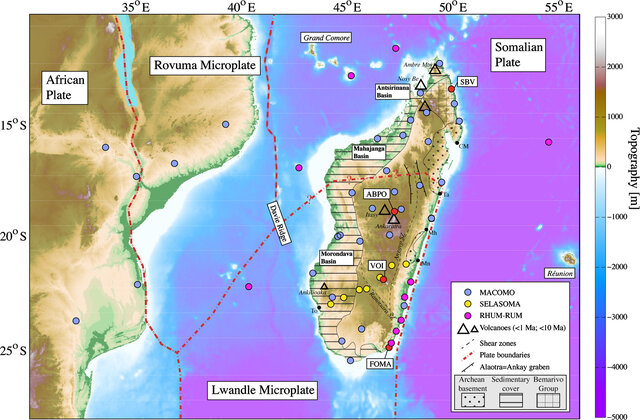
\includegraphics[width=0.5 \linewidth]{./Figures/TopologicMaps/geologyMadagascar.jpeg}
    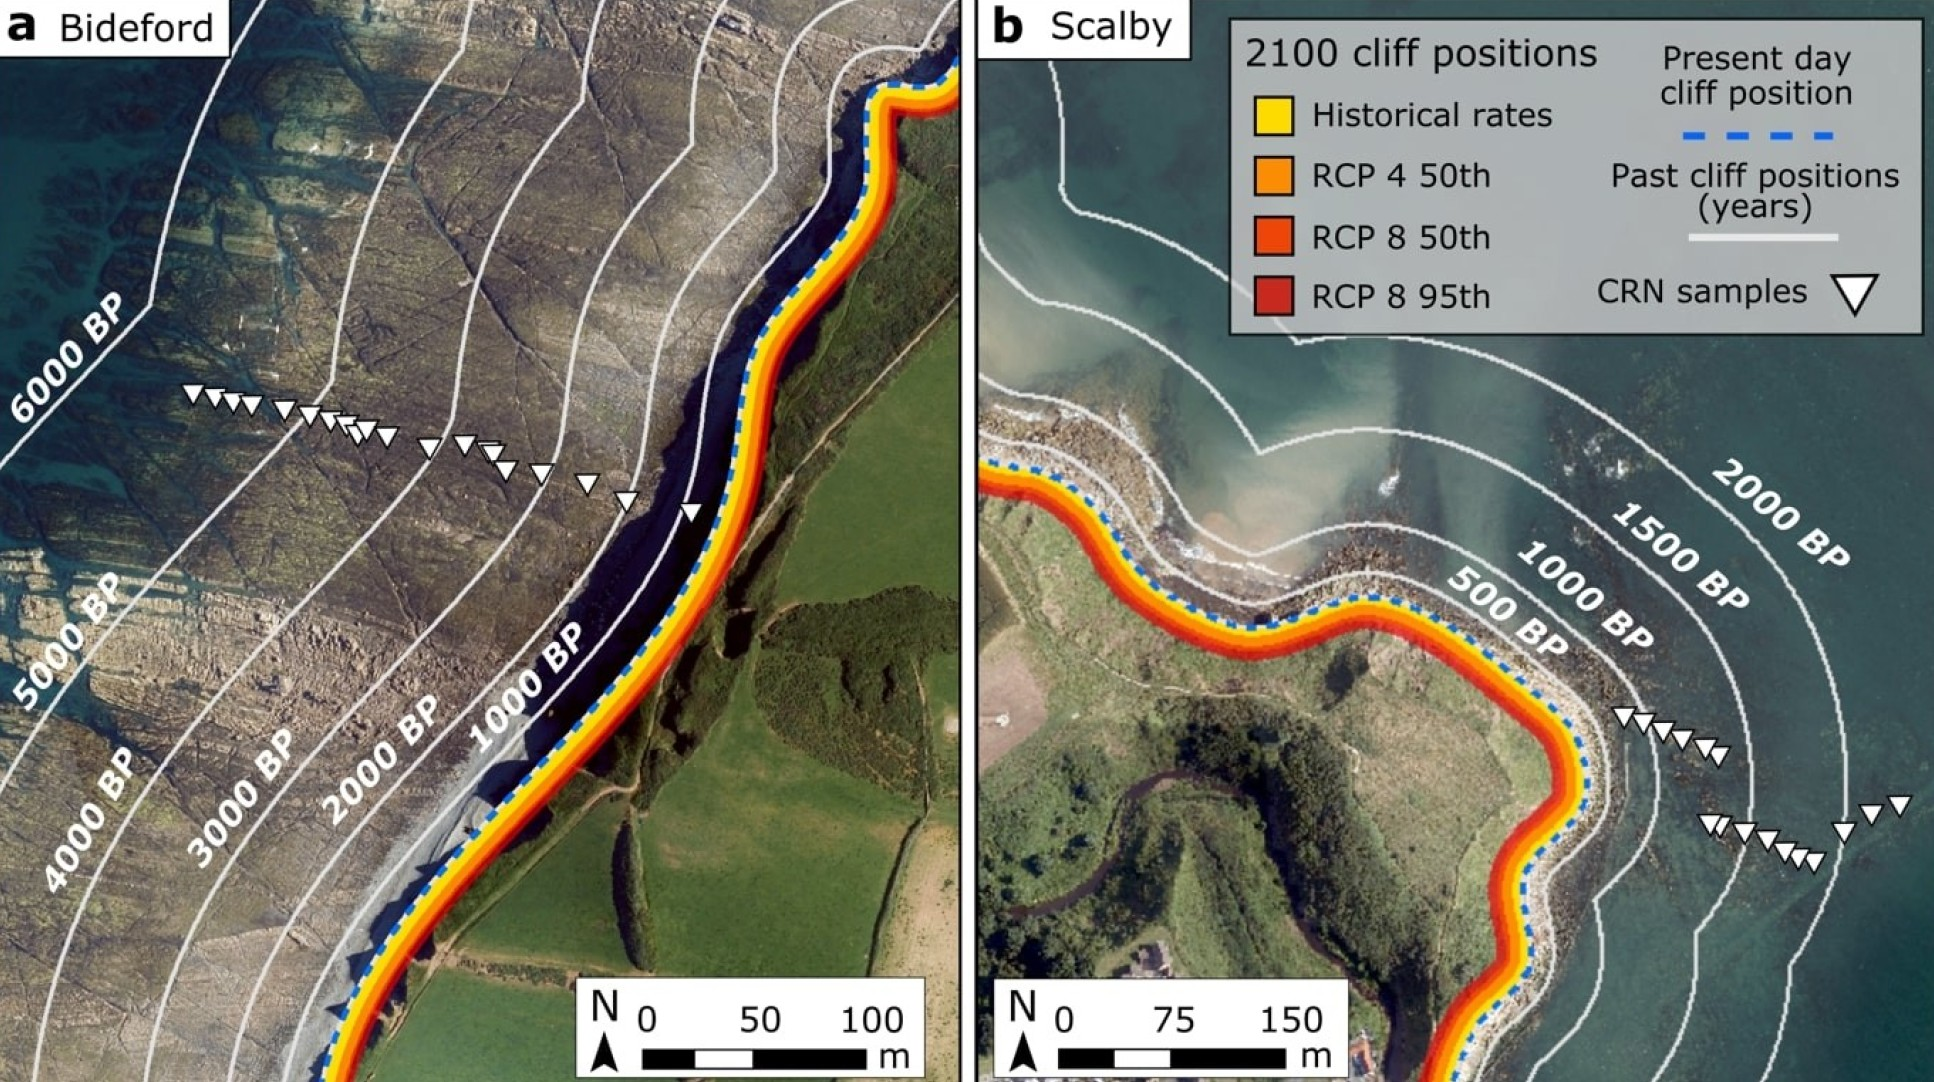
\includegraphics[width=0.5 \linewidth]{./Figures/TopologicMaps/CliffErosionBidefordAndScalby.jpg}
    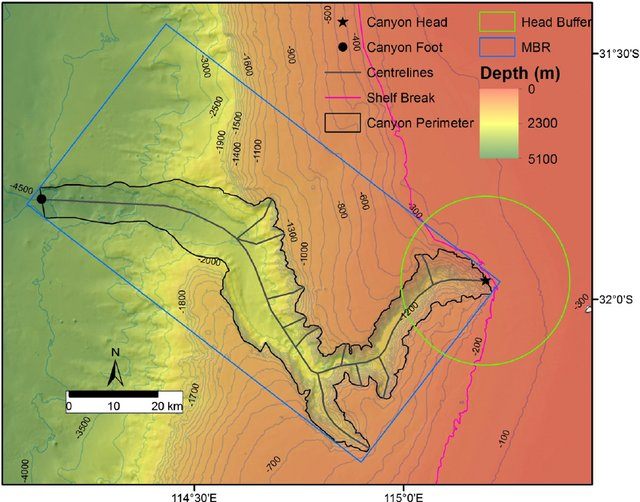
\includegraphics[width=0.5 \linewidth]{./Figures/TopologicMaps/PerthCanyon.jpg}
    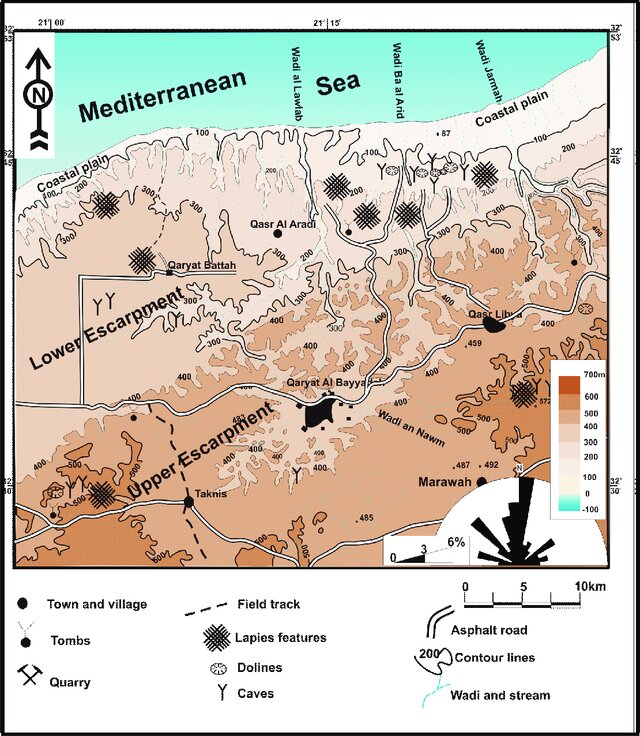
\includegraphics[width=0.5 \linewidth]{./Figures/TopologicMaps/QasrLibya.jpg}
    \caption{Four examples of topographic maps used in earth science. From left to right and top to bottom: Sedimentary distribution other Madagascar island \cite{Pratt2017}, evolution of coastlines at Bideford, UK and Scalby, UK over the last 6000 years and 2000 years respectively (BP = Before Present) \cite{Shadrick2022}, localization of key parameters of Perth Submarine Canyon, Autralia \cite{Huang2014}, and geological features distribution of karstic landscape at Qasr Lybia, Libya \cite{ElAmawy2009}}
    \label{fig:semantic-representation_presentation}
\end{figure}

% Slight introduction
Topographic maps are very useful tools for biologists, geologists or even oceanologists (which would call them "bathymetric charts"). These maps are displayed in 2D but provide 3D information about the altitude (or depth), but can also use symbology to represent the important elements that need to be visible. Map symbols are important in order to extract as much information as possible from a 2D object. In cartography, map symbols are defined as geometric primitives such as points, polylines, polygons, and (more rarely) polyhedrons. These symbols are a simplification of the content of an environment, or an abstraction of the 3D nature of the terrain features as we can see in the examples in \cref{fig:semantic-representation_presentation}. This is useful to understand the relationship between the different features, which may enable to deduce physical rules in the evolution of a terrain. 

% WHo would want it, and why?
In such way, geologists can study the distribution of peaks in a mountain range, the location of soil types in an area, which in turn allow to deduce possible locations of karst networks, for example. Using the same tools, a biologist may interpret the effect of natural or artificial reefs on coastal erosion, or understand more clearly the interactions inside an ecosystem. Oceanologists may also deduce, using the same strategy, the formation of canyons and fans from old river systems. [A REDIRE]

By simplifying the surface details in maps or models, we can concentrate more effectively on gaining a deep understanding of the underlying processes that shape the terrain. This focused understanding allows us to apply the insights we gain to a wide variety of terrain types. Essentially, this approach enables us to generalize our findings and apply them across diverse geographical landscapes, facilitating broader and more versatile applications of our knowledge.

Parallelly, terrain artists most of the time sketch the global shape of the terrain they will model beforehand, such that they can check, before the modeling part, that the consistency and plausibility of the terrain will be valid. Looking at a simplified map before starting the modeling step allows the designer to modify the overall shape of the terrain, at a large scale, before the 3D geometry comes into play, generating too much control points or vertices to be able to deal with.

Starting from an initial configuration or providing conditions on the desired output terrain, the algorithm we propose will let the different terrain features evolve as a multi-agent system in which the user can apply modifications or new constraints on the state of the environment. The resulting configuration is an environment conform to the constraints given by the user over the distribution of features present in the scene.

% Why it does not already exists?
As described in the previous chapter, most terrain generation algorithm use the geometry of an initial terrain surface to iteratively apply changes such as noise-based algorithms or erosion simulation. While the introduction of information about some environment variables or properties of the ground may influence the result of an algorithm, the control of the global shape of the terrain is lost as it treat locally the surface, without knowing which feature a certain point on the surface lies on.

% Personal motivation
The question which led to our solution is the multi-scale user interaction: "Is it possible to provide an interaction mean for terrain generation allowing the user to interact with a small structure like a rock in the same manner as with a large structure like a mountain?". 
In this work, we want the user to be able to have a large scale representation of the terrain in order to generate a landscape that satisfies his needs while keeping the possibility to apply large modifications.
In discussion with robotician users, we realise that we want to create a large landscape that can contain interesting configurations, select a smaller region that may have features in a disposition that fits its requirements and then refine again the given region.
In the optic of generating a large scale terrain in which we could focus the generation effort in a certain region, we wished to be able to see a coarse representation that can be computed quickly.

We aim for our terrain generation method to be versatile enough to handle both terrestrial and aquatic environments. This dual capability would allow the method to be applicable to landscapes above the water level, such as mountains and valleys, as well as to submerged terrains, such as oceanic canyons and coral landscapes.

Because many geographical terms and computer science terms are deceptive cognates, we will try to find middle ground in the naming of our introduced structures to avoid as much as possible any ambiguity between the research fields.
% Because many geographical terms would become ambiguous in computer science terms, in which this thesis lie in, we will translate some vocabulary in a way that may be disapproved by geologists, but we are doing our best to keep it as acceptable for each field as possible.


% \subsection{Nomenclature}
% % Geographical feature/entity -> Semantic Terrain Entity
% A geographical feature, also known as a feature, object, or entity, is a discrete phenomenon located at or near the Earth's surface, relevant in geography and geographic information science. It represents geographic information that can be depicted in maps, geographic information systems (GIS), and other forms of geographic discourse. The term "feature" includes both natural and human-made objects, ranging from tangible items like buildings to intangible concepts like neighborhoods. Features are distinct entities with defined boundaries, differentiating them from continuous geographic masses or processes occurring over time. They can be categorized as natural features, such as ecosystems, biomes, water bodies, and landforms, or artificial features, such as settlements, administrative regions, and engineered constructs. Geographic features are described by characteristics including identity, existence, classification, relationships with other features, location, attributes, and temporal aspects. Information about these features is stored in geographic databases using models like GIS datasets, which organize and represent these features in structured formats.
% % A geographical feature, also referred to as a feature, object, or entity, is a discrete phenomenon located at or near the Earth's surface, relevant in geography and geographic information science. It is an item of geographic information that can be represented in maps, geographic information systems (GIS), remote sensing imagery, statistics, and other forms of geographic discourse. The term "feature" is broad and inclusive, encompassing both natural and human-made objects. It includes tangible items like buildings as well as intangible concepts like neighborhoods. Features are discrete entities with distinct identities and locations, characterized by defined boundaries that differentiate them from other objects, distinguishing them from geographic processes, which occur over time, and geographic masses or fields, which are continuous. In geographic information science, "feature," "object," and "entity" are often used interchangeably, although some formal distinctions exist, such as seeing a feature as an abstraction of a real-world phenomenon. Geographical features can be categorized into natural and artificial types. Natural features include ecosystems, which are communities of organisms interacting with their environments; biomes, which are large areas with ecologically similar communities defined by plant structures, climate, and ecological patterns; water bodies, which are significant accumulations of water like oceans and lakes, either distinct or conceptual in nature; and landforms, which are physical structures such as mountains and valleys defined by surface form, location, and topography. Artificial features encompass settlements, which are human communities ranging from small villages to large cities, including infrastructure like roads and buildings; administrative regions, which are social constructs like states and neighborhoods used for organizational purposes; engineered constructs, which are man-made structures such as highways and airports; and cartographic features, which are abstract map representations, such as grid lines and boundaries, that do not physically exist. Geographic features are represented by descriptors of their characteristics, including identity, existence, kind, relationships, location, attributes, and time. Each feature is unique, often identified by names or codes, and its existence refers to its presence in the real world, including features that are proposed or planned. The kind refers to its classification, such as a building or river, while relationships describe spatial, meronomic (part-whole), and genealogical (parent-child) connections with other features. The location provides a description of where a feature is, including its shape and extent, and attributes describe other characteristics, such as population or size, often expressed as text or numbers. Time relates to the temporal aspects of a feature's characteristics, describing changes over time. Information about features is stored in geographic databases, often using vector data models, including GIS datasets, which help represent these features and their various descriptors in a structured format.

% % Field -> Environmental Attribute
% In geography, the term "field" refers to a continuous spatial phenomenon defined across a region, where each point in that region has a specific value of some variable. Unlike discrete objects, which have distinct boundaries and identities, fields represent variations of phenomena occurring over a continuous space, such as temperature, elevation, or precipitation. Fields can be either scalar or vector quantities: scalar fields represent a single value at every point, like temperature, humidity, or elevation, while vector fields represent quantities with both magnitude and direction, such as wind velocity or ocean currents. Examples of fields in geography include topographic fields, where elevation values are distributed across a landscape; climatic fields, where temperature or precipitation values are mapped over a geographic area; and magnetic fields, which capture the intensity and direction of magnetic forces at various points on the Earth's surface. Fields are often represented mathematically using functions or equations that define how the field's value varies over space, including interpolation or modeling techniques to estimate field values at unsampled locations. In Geographic Information Systems (GIS), fields are typically represented as raster data, where a grid of cells captures the continuous variation of a field across a landscape, with each cell holding a value representing the field's magnitude at that location. Fields are crucial for spatial analysis and modeling, allowing geographers to study patterns and processes that vary continuously across space, such as climate change, land surface modeling, and resource distribution. Thus, in geography, a field is a method of representing continuous spatial phenomena, enabling the analysis of patterns and trends across geographic spaces.

% % Event -> Geological Event
% In philosophy, an "event" is defined as an occurrence or happening that takes place at a specific time and location, characterized by its temporal nature and involvement in change or transition. Unlike static objects, events are dynamic and are often considered fundamental constituents of reality. They typically involve transformations from one state to another, such as a tree falling, and are central to discussions about causality, as they can serve as causes or effects within causal chains. Philosophers debate whether events are basic entities or reducible to other kinds of entities, like properties of objects or states of affairs. They also explore how events are individuated and identified, what distinguishes one event from another, and how events relate to objects. Linguistic and logical analyses focus on how events are described in language, often through verbs and predicates, and how they relate to entities involved. Various philosophical theories, such as process philosophy, emphasize events over static entities, offering different frameworks for understanding the nature of events and their role in the structure of reality. Overall, events are crucial for understanding change, causality, and our perception of the world.

% % Visualization

% \subsection{Features on field experts maps}
% - ... 
% \subsection{Topographic/Planimetric maps}
% - ... 

% \subsection{Analogy}
% - Compare our nomenclature with introduction \\
% - ... 

\section{State of the art}
\label{sec:semantic-representation_related-works}

\subsection{Vector modeling}
...
\subsubsection{Implicit modeling}
...
\subsubsection{Diffusion models}
...

\subsection{Ecosystems simulation}
...
\subsubsection{Environment modeling}
...
\subsubsection{Individual process}
...
\subsubsection{Multiple entity simulation process}
...
\subsubsection{Cellular automata}
...

Procedural terrain generation has been heavily studied for the last 40 years \cite{Galin2019}. Researches in this topic try to find new solutions to compromise between realism, user control and efficiency \cite{Gain2009}. Using fractal noise parametrized to resemble real landscape has been an important first step \cite{Musgrave1989} as it's a fast and light solution to generate procedurally the appearance of mountains. The lack of user control pushed newer works toward the use of controlled noise by including real DEM in the process through learning \cite{Kapp2020}, while the rise of deep learning technologies gave higher control to the user through sketches \cite{Guerin2017, Talgorn2018}.

All the algorithms aim to reproduce plausible relief in terrestrial landscapes, mostly limited to alpine landscapes, but a lack of research can be found in almost all other biomes \cite{Smelik2014}. Underwater landscapes generation, for example, has been almost completely absent from literature for many reasons: the difficulty of accessing the area, the lack of visibility under water and the complex physics of underwater geology and biology make the algorithms adapted for this environment scarce. 

While stochastic noise can be sufficient to model coarsely the ocean floor \cite{Mareschal1989}, this process won't cover areas with the biggest biomass, near shallower waters such as near coasts and islands. These areas, that represent a very small portion of the oceanic surface, are much more complex as many interactions between biolife, air and water are in action.

Due to the impossibility to observe the large-scale and the small-scale of underwater environments, some works related to geology model large structures like the profile shape of the coral reef \cite{Bosscher1992}, simulate its surface growth \cite{Li2021}, or use procedural algorithms for single coral colonies' growth simulation \cite{Abela2015}. We however don't have a mix of the different scales, and neither methods take into account the environment such as the topography or the interaction of different terrain features. This is mainly due to the fact that the evolution time for each scale varies from a span of weeks to thousands of years.

Recent works have been presenting "feature tools" to correct landscapes from unaccurate DEM (2.5D) using vector-based features that modifies the geometry of the ground and water bodies to fit thir respective 2D satellite images, by explicitely defining the position of natural features like rivers and mountains \cite{Ketabchi2016}. Visible 3D features like vegetation and buildings can also be added in the final result as meshes affected to a single point. This leads to sketch-based applications where features are represented like topographic maps. This solution allows for the manipulation of an existing terrain, guided by a real-world satellite image, but lacks the possibility to completely generate an unseen landscape or for the terrain features to interact between them. Feature tools have been proposed to generate terrains from scratch \cite{Smelik2010a}, but usually require to define in advance the interactions between each feature like a automatically displaying a bridge when a river crosses a road.

In an ecosystem, every element within the system has an impact on its surroundings, and accurately simulating physical properties like shading, heat, and humidity can require immense computational power. To address this, instead of simulating these properties individually for each object, they can be represented as scalar fields that span the entire scene. These scalar fields, which may represent temperature, humidity, or occlusion, are locally influenced by nearby objects and terrain features, such as trees casting shadows or buildings radiating heat. This approach, as described in \cite{Grosbellet2016, Guerin2016a}, allows for the environment's physical properties to be computed in a more efficient manner. By simplifying the complex interactions into these localized scalar fields, they called environmental objects, their method provides a scalable system that can handle large and detailed scenes. This system effectively renders scene details, such as snow accumulation or leaf distribution, in a way that is visually plausible, ensuring realistic results without the need for exhaustive simulations. 
%In a similar way, other works represent the wind flow as a composition of local vector fields \cite{Wejchert1991}, avoiding complex fluid simulation while providing user control in a lightweight model. We extend these works by incorporating a time-evolution system such that the scene can be dynamic.
In a similar approach, parallely Wejchert and Haumann \cite{Wejchert1991} and Sims \cite{Sims1990} represent wind flow as a composition of local vector fields, known as "flow primitives", which can be combined to simulate complex fluid behavior. This method simplifies the computation by avoiding full fluid simulations, instead offering a lightweight model that allows for intuitive user control over the flow dynamics.
By combining these approaches, we can create dynamic ecosystems where environmental effects and fluid flows interact in a plausible manner, while requiring a low computation effort and preserving a high user control.


\section{Description of the method}
\label{sec:semantic-representation_pipeline}

In this section, we present the pipeline and processes that underpin our method. Our approach introduces the concept of \glosses{EnvObj}, simplified terrain features that interact with their surroundings to simulate complex ecosystem dynamics. These \glosses{EnvObj}, which can represent natural features such as trees, rivers, or rocks, influence and are influenced by scalar fields like temperature, humidity, and elevation. The method is structured into several key phases: initialization, where the foundational elements of the terrain and \glosses{EnvObj} are set up; an iterative generation process, where these \glosses{EnvObj} are instantiated and interact with their environment; and finally, the production of a sparse representation of the scene's features. This section details each of these phases, explaining how the system dynamically adapts to user input and environmental changes.

\subsection{Pipeline}

\begin{figure*}
    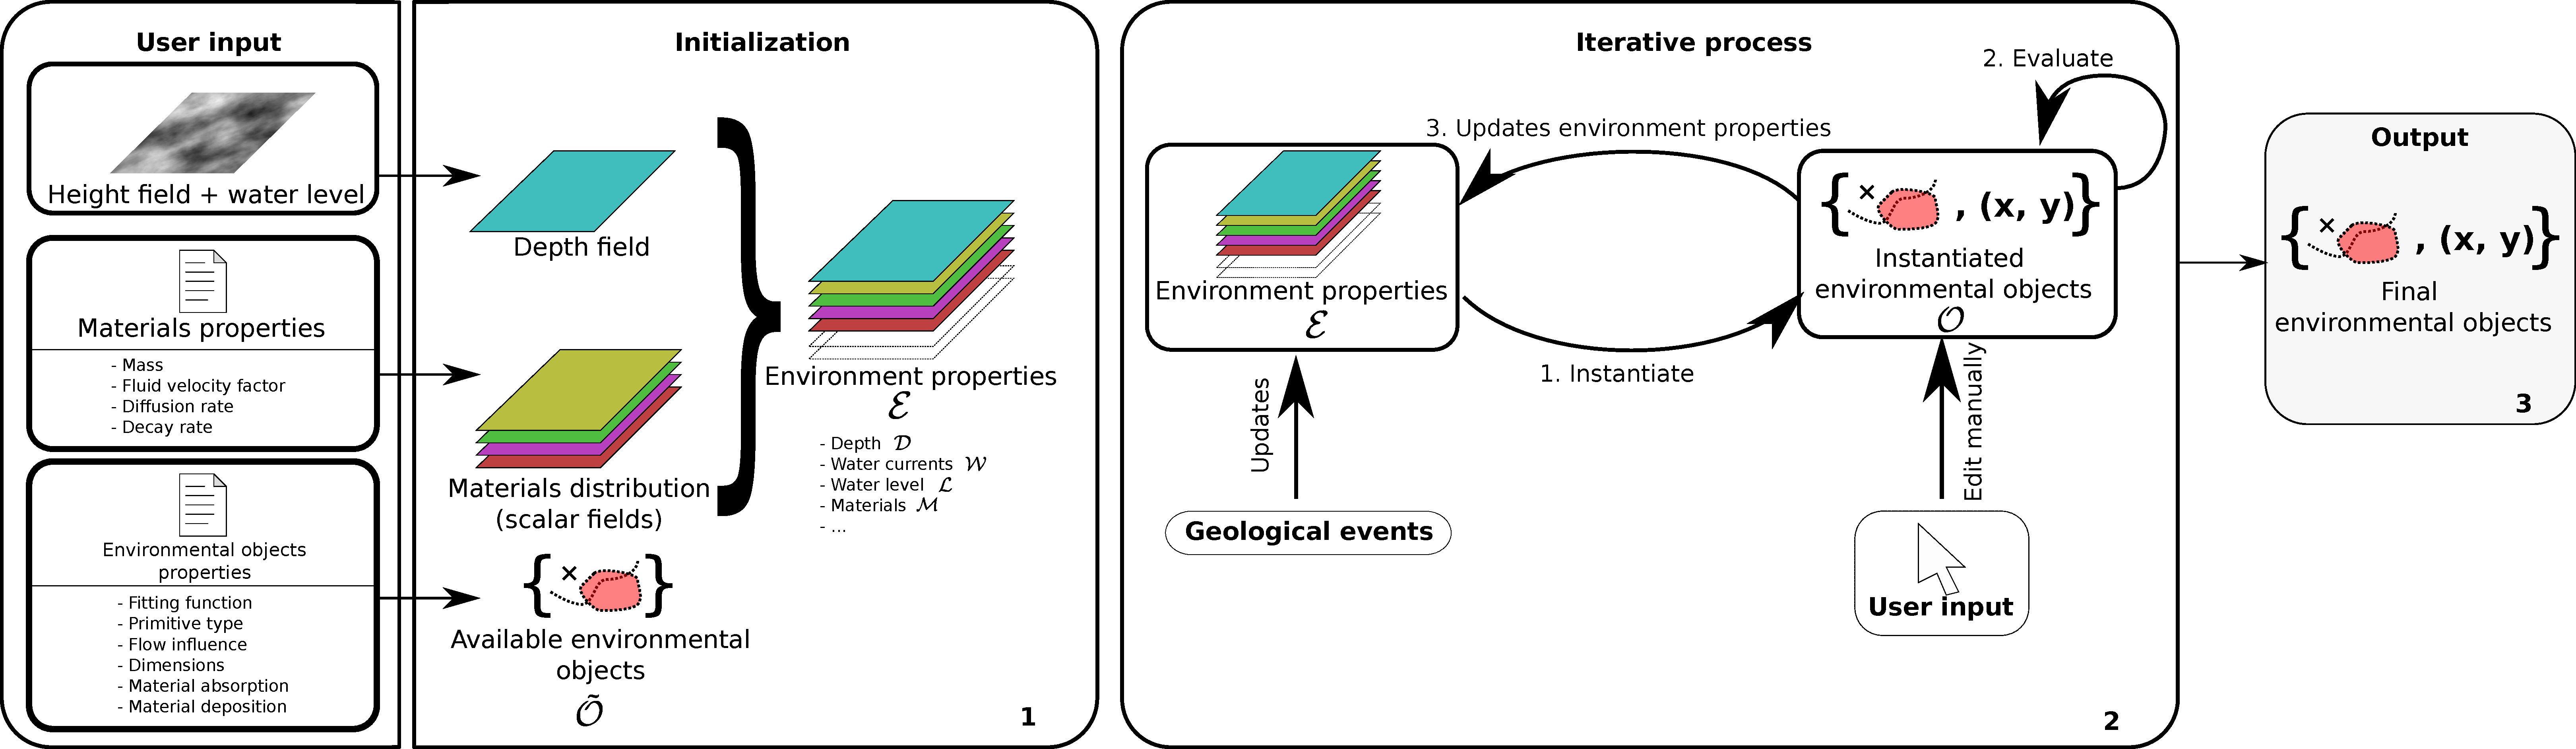
\includegraphics{Figures/pipeline.pdf}
    \caption{Overview of the pipeline of the method. The user provides as input an initial height field and sets the water level, as well as a definition of the \glosses{EnvMat} properties and \glosses{EnvObj} properties that will be used in the iterative process. These inputs are initialized as an initial set of \glosses{EnvObj} and scalar fields that represents the \glosses{EnvVal}. In the iterative loop, new \glosses{EnvObj} are instantiated using the current state of the environment at their optimal position. The existing \glosses{EnvObj} in the terrain reevaluate their \gloss{FitnessFunc} to grow or die and update the \glosses{EnvVal} locally. At each iteration, \glosses{GeoEvent} can update the \glosses{EnvVal}, while the user can interact directly with the \glosses{EnvObj}. The result of the whole process is a set of \glosses{EnvObj} which is a sparse representation of the features of the scene. }
    \label{fig:semantic-representation_pipeline}
\end{figure*}

\subsubsection{Initialization}

The generation of the terrain is initialized using an initial height field $h$ and an initial water level $\Wlevel$. 
During this chapter we will include many features depending on altitude or depth, so we will use the shorthand notations $\height = h - \Wlevel$ and $\depth = -\height$. The height field provides variation on the altitude, which can influence the generation process of the scene.

The list of available \glosses{EnvObj} $\availableObjects$, representing the different features that can be present in the scene, are provided with their properties: type, size, \glosses{GenRule} and effects on the \glosses{EnvVal} (\cref{sec:semantic-representation_environmental-objects}). A target list of \glosses{EnvObj} $\targetObjects$ can be defined to control the final result of the generation.

Finally, different \glosses{EnvMat} are defined with their properties such as diffusion speed, mass, decay rate and influence from the water currents. An initial environment configuration resulting from the initial height field $\height$ and water level $\Wlevel$, the \glosses{EnvMat} distribution $\material$ (represented as scalar fields $\material: \R^2 \to \R$) and water currents $\Water$ (as a vector field $\Water: \R^2 \to \R^2$) will be used by the \glosses{EnvObj} of the scene to simulate their growth and spawn at the most probable position. The \glosses{EnvVal} are noted $\environment = (\depth, \Water, \Wlevel, \material)$ (\cref{sec:semantic-representation_communication}).

The definition of \glosses{EnvObj}' properties and \glosses{EnvVal} is done with field experts, providing the pertinent parameters required to model the evolution of the terrain features using expert knowledge (\cref{sec:semantic-representation_biology}). 

The generation phase starts with an initial set of \glosses{EnvObj} present in the scene, which can optionally be pre-filled.

\subsubsection{Generation process} 

%- Main loop
Once the initialization phase is done, the generation begins. The generation process is incremental and its main loop is composed of two different steps: the instantiation of new \glosses{EnvObj} then the update of the environment. This loop is repeated until the user is satisfied with the look of his environment or following rules like a number of features threshold or a targeted list of \glosses{EnvObj} as described in the layout planner defined in \citep{Tutenel2009}.


\subsubsubsection{Instantiation}
% - Object instantiation
At each iteration, new \glosses{EnvObj} can be created at their most fitting locations if possible. The \glosses{GenRule} provided in the initialization phase are used to find an optimal position from stochastic sampling (\cref{sec:semantic-representation_generation-rules}). 
All \glosses{EnvObj} are evaluating their state analytically using a \gloss{FitnessFunc} and a \gloss{FittingFunc} provided as input (\cref{sec:semantic-representation_generation-rules}).

\subsubsubsection{Environment update}
% Once the new objects are instantiated, the process can continue.
% - Environment update
Once the instantiation step is done, the \glosses{EnvVal} are updated by each \gloss{EnvObj} through \glosses{EnvModif}, which depose and absorb some of the \glosses{EnvMat} $\material$ (\cref{sec:semantic-representation_materials}) while modifying the water currents $\Water$ (\cref{sec:semantic-representation_water-currents}) and the height field $\height$ around them. Finally, water currents and terrain slope displace \glosses{EnvMat} of the terrain until reaching a dynamic equilibrium in the environment at each iteration.

% We consider the water currents to be a steady-state flow, allowing us to remove the variation from time in the flow equations.
% The water currents are updated locally by each \gloss{EnvObj} using an analytical form $W^*(\p) = W(\p) + \omega(\p)$.
During the generation process, the user can alter directly the distribution and shapes of the \glosses{EnvObj} (\cref{sec:semantic-representation_manual-interaction}) and perturb the generation process by planning \glosses{GeoEvent} that have impacts on the \glosses{EnvVal} (\cref{sec:semantic-representation_events}).


\subsubsection{Output}
% - Output result
The output of our system is a set of \glosses{EnvObj} disposed in the plane. We do not provide the 3D representation of the \glosses{EnvObj} in this chapter, letting the user define the rendering method. The figures used in the chapter use a mix of implicit surfaces and triangular meshes.

\subsection{\Glosses{EnvObj} }
\label{sec:semantic-representation_environmental-objects}
A geographical feature, also called object or entity, is defined as a discrete phenomenon located at or near the Earth's surface, relevant in geography and geographic information science (GIScience). It represents geographic information that can be depicted in maps, geographic information systems (GIS), and other forms of geographic media. This term includes both natural and human-made objects, ranging from tangible items like buildings or trees to intangible concepts like neighborhoods or savana. Features are distinct entities with defined boundaries, differentiating them from continuous geographic masses or processes occurring over time. They can be categorized as natural features, such as ecosystems, biomes, water bodies, and landforms, or artificial features, such as settlements, administrative regions, and engineered constructs. Geographic features are described by characteristics including identity, existence, classification, relationships with other features, location, attributes, and temporal aspects. Information about these features is stored in geographic databases using models like GIS datasets, which organize and represent these features in structured formats. As the term "feature" is overused in computer science, we will use the term \gloss{EnvObj} in this work.

Each \gloss{EnvObj} is shaped with a simple geometric shape called a "skeleton" that defines where it is located and how it fits into the environment. The \gloss{Skeleton} can either be, as used in cartography, a point, a curve or a region. We will then refer to our \glosses{EnvObj} as point-based, curve-based or region-based, respectively.  
These \glosses{EnvObj} interact with the environment $\environment$ by changing local conditions using the \glosses{EnvModif}. For example, the presence of a river might increase the moisture in the surrounding area, while a mountain might induce more rockiness in the soil composition. They can also absorb changes from the environment, such as a forest taking in humidity from the air.
The placement of \gloss{EnvObj} is determined by a \gloss{FitnessFunc} $\fitnessFunc$, which evaluates how suitable a location is based on the \glosses{EnvVal}. Once a suitable location is found, the \gloss{FittingFunc} optimizes the shape and position of the entity to fit as best as possible into the environment $\fittingFunc$.

%This approach allows us to "spawn" new entities based on rough altitude estimates, ensuring that their placement is contextually appropriate while deferring the detailed computation of their final shape to a later stage, if required by the user.
% The coarse height function thus acts as a middle between the semantic modeling of terrain and the precise 3D modeling. It provides enough information to make informed decisions about \glosses{EnvObj} placement and \glosses{EnvMat} while preserving the flexibility to integrate more detailed modeling techniques. This method ensures that the terrain generation remains interactive and scalable, allowing for the dynamic and realistic placement of entities in complex landscapes without being tied to the immediate computation of detailed topography.

% \Glosses{EnvObj} are rule-based objects following rules depending on their local environment for evaluation their state in their life cycle. We can see them as a life form in the way that they are created and eroded with time. During their lifetime, they influence their local environment by depositing and absorbing \glosses{EnvMat} around them and influencing the water currents. The environment objects are described spatially as a single point, a parametric curve or a region.


\subsection{\Glosses{EnvVal} }
\label{sec:semantic-representation_communication}

In geography, a "field" refers to a continuous spatial phenomenon across a region where each point has a specific value of a variable, unlike discrete objects with distinct boundaries. Fields can be scalar, representing a single value at every point (like temperature or elevation), or vector, representing quantities with magnitude and direction (like wind velocity). Examples include topographic fields for elevation, climatic fields for temperature or precipitation, and magnetic fields for magnetic forces. Because of the ambiguous nature of the term "field" with mathematics and computer science, we will define the geographic fields as \gloss{EnvVal}.

In an ecosystem simulation, each actor of the ecosystem has an impact on all other actors, which results in an exponentially growing computation effort as the number of elements of the terrain increase. We avoid this problem by considering the \glosses{EnvVal} as a proxy to allow any \gloss{EnvObj} to interact with any other one. Each of the \gloss{EnvObj} have a local impact on the \glosses{EnvVal} without knowledge of neighboring \glosses{EnvObj}. This modification of the \glosses{EnvVal} are presented as the effect of \glosses{EnvModif} defined for each \gloss{EnvObj}. % can be due to an absorption and deposition of some material $\material$ or an influence on the water currents.

In this work, we have integrated vector \glosses{EnvVal} (e.g., water currents $\Water$) and scalar \glosses{EnvVal} (e.g., altitude $\height$, water level $\Wlevel$, and various material properties $\material$) under the unified term "environment," denoted as $\environment = \left( \height, \Water, \Wlevel, \material \right)$. The \glosses{EnvMat} represent abstract quantities such as the availability of sand, salt, moisture, or rocks at each point. It is important to emphasize that these materials are not to be visualized as physical layers stacked on the terrain surface. Instead, they should be understood as conceptual resource distributions that influence the environment and the behavior of \glosses{EnvObj}, rather than as something directly observable in the scene.

\subsubsection{\Glosses{EnvModif} $\environmentModif$}
The environment determine if a \gloss{EnvObj} does belong at a certain position. When a \gloss{EnvObj} is placed, its surrounding \glosses{EnvVal} can be affected though \glosses{EnvModif} noted $\environmentModif = (\heightModif, \waterModif, \nothing, \materialModif)$ defining a change of height $\heightModif$, changes in the water currents $\waterModif$ and \gloss{EnvMat} alteration $\materialModif$. 

\Glosses{EnvObj} are subject to altitude conditions. However, to maintain a clear distinction between semantic modeling and 3D modeling, we do not compute the exact physical shape or detailed height field of each \gloss{EnvObj}. Instead, we define a \gloss{CoarseHeight}, a parametric representation derived from the \gloss{Skeleton} to provide a rough estimate of the changes in elevation around it. This simplified model of how the \gloss{EnvObj} influences the surrounding terrain's altitude allows us to cheaply evaluate the potential presence of new entities that have altitude-dependent conditions without the need to perform expensive computations to generate a detailed height map of the entire terrain. 

Altering the vector field of the water currents $\Water$ is done by the composition of the effect $\waterModif$ of each object at a position $\p$ as introduced in \citep{Wejchert1991}, while we use the formulation of Kelvinlets \cite{DeGoes2017} in the computation of effect of each \gloss{EnvObj}.

Each \gloss{EnvObj} has intrinsic \glosses{EnvMat} that can be seen as "spreading" and "absorbed" around its skeleton over time. A coral reef may produce coral polyps and at the same time reduce the water currents. It grows thanks to the deposition of limestone from coral colonies. In our model, the colonies affect the \glosses{EnvVal} through the deposition of \gloss{EnvMat} $\materialModif_\text{limestone}$, which in turn, is absorbed by the coral reef, without a direct exchange between the two \glosses{EnvObj}.

The alteration of a scalar \gloss{EnvVal} is done by adding or removing some amount around the \gloss{Skeleton} of the \gloss{EnvObj} and diffusing it in the space, influenced by the water currents. We consider the system to be \gloss{SteadyState}, garantied by the introduction of a decay rate $\decay > 0$ in the computation of the diffusion and advection.



\section{Placement of \glosses{EnvObj} in an environment}
\label{sec:semantic-representation_generation-rules}

At each iteration of our algorithm, we want our \glosses{EnvObj} to be at plausible positions. We do not guaranty a temporal continuity between iterations as in \citep{Ecormier-Nocca2021}, so the objective is to add new \gloss{EnvObj} in order to satisfy the users wishes, while conserving the plausibility of the scene. Rather than "forming" these \glosses{EnvObj}, our method "reveals" them, much like a paleontologist uncovers fossils during an excavation. A paleontologist does not dig randomly across the Earth to find fossils; instead, they analyze the geological context to identify the most likely locations. Similarly, our method observes the environment and estimates where certain elements are likely to exist. For example, in hydrology, if a river appears to originate from nowhere, it might suggest the presence of a karstic river system upstream. In urban planning, if many roads converge at a certain point, it is reasonable to expect that a city is located there. This approach ensures that Semantic Terrain Entities are revealed in positions that are contextually appropriate and coherent within the landscape.

We will follow the same intuition using a \gloss{FitnessFunc} for each of the \gloss{EnvObj} that may be spawn in the terrain. The \gloss{FitnessFunc} defined $\fitnessFunc: \environment \to \R$ provides a score indicating how well the \gloss{EnvObj} may fit in this position. Evaluating this function at multiple position results in an approximation of the fitness map of the entity. Once the most probable position is found, we can find the most plausible shape of the \gloss{EnvObj} using the \gloss{FittingFunc} $\fittingFunc$.

For this task, we place a new elements required at the most plausible position using the analysis of the \gloss{FitnessFunc} of each \gloss{EnvObj}. We know that each \gloss{EnvObj} will modify the environment surrounding, which may make previously instantiated \glosses{EnvObj} unfitted. Knowing this,the goal is to add the new element at the position that will change the least the stability of the system. 

Genetic algorithms or Depth First Search algorithms could be used to try many possibilities until a local or global minimum could be found, but this would require a large processing power. Naive genetic algorithms would place a \gloss{EnvObj} at a certain position at each iteration and evaluate the stability of the environment, repreating this operation while varying slightly the position of the \glosses{EnvObj} or the type of \gloss{EnvObj} instantiated at each iteration, resulting in way too much computation to stay interactive. The Depth First Seach algorithms would require to compute all the possible combinations of \glosses{EnvObj} and positions which, given the fact that we want a continuous position in order to work multi-scale, would require to compute an incredibly high amount of possible configurations in order to find a plausible situation, on average. We will work with an evolutionary algorithm to find a compromise between fast computation and a satisfying result.

Our placing algorithm is done in two steps: first, it identifies the global location where a \gloss{EnvObj} best fits within the environment $\environment$ using its \gloss{FitnessFunc} $\fitnessFunc$, which evaluates the suitability of each point $\p$ based on the \glosses{EnvVal} $\environment_p$, including factors such as altitude $\height(\p)$, water current velocity and direction $\Water(\p)$, water level $\Wlevel(\p)$, and the availability of \gloss{EnvMat} $\material(\p)$. Second, once the most suitable location is identified, the algorithm determines the most plausible shape of the \gloss{EnvObj} using the \gloss{FittingFunc} $\fittingFunc$.

To ease the reading the functions $\fitnessFunc(\environment(\p))$ and $\fittingFunc(\environment(\p))$ with $\environment(\p)$ the \glosses{EnvVal} at the point $\p$ of the terrain are simplified to $\fitnessFunc(\p)$ and $\fittingFunc(\p)$ respectively.

% Our placing algorithm is done in two steps: first we estimate at which global location the \gloss{EnvObj} fits the most given an environment $\environment$ using its \gloss{FitnessFunc} $\fitnessFunc$, secondly we estimate the shape of the skeleton of this \gloss{EnvObj} should take given a \gloss{FittingFunc} $\fittingFunc$.

% \Glosses{GenRule} provides, for each \gloss{EnvObj}, a \gloss{FitnessFunc} $\fitnessFunc$ defining the most probable location for an \gloss{EnvObj} to be found. \Glosses{FitnessFunc}' parameters contains, for every point $\p$, the \glosses{EnvVal} $\environment_p$ (the altitude $\height(\p)$, the velocity and direction of the water currents $\Water(\p)$, the water level $\Wlevel(\p)$ and the amount of each \gloss{EnvMat} available $\material(\p)$).

\subsection{\Gloss{FitnessFunc} }
"Darwinian fitness" refers to an organism's ability to survive and reproduce in its environment. It is a measure of how well-suited an organism is to its surroundings, and those with higher fitness are more likely to pass on their genes to the next generation. In a similar vein, the \gloss{FitnessFunc} of a \gloss{EnvObj} evaluates its suitability at a location in the terrain, extending the meaning to living features like forests and corals and non-living elements such as rivers, mountains, karsts, etc.

The fitness function is constructed by evaluating several environmental variables at a given location $\p$. These include altitude ($\height(\p)$) and its gradient ($\nabla \height(\p)$), the availability and gradient of various materials ($\material_i(\p)$ and $\nabla \material_i(\p)$), water current characteristics ($\Water(\p)$), and water level ($\Wlevel(\p)$). Altitude and its gradient can influence the placement of objects like rivers, which may prefer lower elevations, or forests, which might thrive on slopes. Each material, such as limestone, sand, or clay, is considered separately, and their availability and gradients at a location are crucial for determining the suitability of different \glosses{EnvObj}, such as a coral reef requiring specific substrates. The velocity and direction of water currents are essential for placing aquatic features or determining where erosion might occur, while the proximity to water influences the likelihood of placing wetlands, lakes, or other hydrological features.

% These environmental variables are typically combined in the fitness function, often expressed as a weighted sum, but not restricted to this form:

% \begin{align*}
%     \fitnessFunc(\p) = w_1 \cdot \height(\p) + w_2 \cdot \nabla \height(\p) + \sum_{i} \left( w_{3,i} \cdot \material_i(\p) + w_{4,i} \cdot \nabla \material_i(\p) \right) + w_5 \cdot \Water(\p) + w_6 \cdot \Wlevel(\p)
% \end{align*}

% Here, $w_1, w_2, w_{3,i}, w_{4,i}, w_5, w_6$ are weights that reflect the relative importance of each factor for the specific \gloss{EnvObj} being considered.

Different types of \glosses{EnvObj} require different criteria for their fitness evaluation. For example, a river might prioritize lower altitude and proximity to water currents, while a forest might prioritize higher altitude and specific material availability. The flexibility of the fitness function allows it to be customized for each \gloss{EnvObj}, ensuring that the generated terrain remains coherent and realistic.

\subsection{\Gloss{FittingFunc} }
The seed point of a spawning \gloss{EnvObj} is defined at the point $\p$ satisfying $\arg \max_\p \fitnessFunc(\p) $.
% a stochastic sampling of the plane. We propose different optimization means to find the optimal fitting position, depending on the \gloss{EnvObj} shape.

\subsubsection{Point-based \gloss{Skeleton}}
The spawning position of a punctual \gloss{EnvObj} is found at the local maxima of the \gloss{FittingFunc} from the seed point. While the \gloss{FittingFunc} doesn't have to be identical to the \gloss{FitnessFunc}, we usually use $\fittingFunc = \fitnessFunc$ for point-based \glosses{EnvObj}. If the two functions are different, the optimisation process simply follows the field's gradient $\nabla \fittingFunc$ until the local maxima is reached.

\subsubsection{Curve-based \gloss{Skeleton}}
% A curve can have different \glosses{GenRule}, making the definition of the functions easier depending if the \gloss{EnvObj}'s \gloss{Skeleton} has a notion of direction. It can either:
% \begin{itemize}
%     \item follow the gradient of the \gloss{FittingFunc} $\nabla \fittingFunc$, useful when the direction of the \gloss{Skeleton} has an importance like a river that has to run downhill,
%     % \item follow the isocontour $\nabla \fittingFunc^\perp$, [WAIT, IS THAT NEEDED?]
%     \item or optimize the energy of the function over its curve, like a coral reef that has to cover as much coral colonies as possible. % follow the heat points.
% \end{itemize}

% \subsubsubsection{Following the gradient}
% Following the gradient of the \gloss{FittingFunc} $\nabla \fittingFunc$ is done by extending a curve from the seed point towards $\nabla \fittingFunc$ until reaching a local maximum while also following $-\nabla \fittingFunc$ until finding a local minimum. We stop the building process when our curve reaches a length limit $\Length$. 

% This \gloss{FittingFunc} strategy is efficient to describe rivers as we can set $\fittingFunc(\p) = \height(\p)$ to force it to always run downstream. 

% \subsubsubsection{Energy optimization}
The skeleton of a curve-based \gloss{EnvObj} is determined by the shape that fits the most given the environment it is added to. 
Using a modified version the Active Contours algorithm \cite{Kass1988}, we can minimize the energy $\energy$ for the parametric curve $\curve$ given $\energy(\curve) = \Einternal + \Eexternal + \Eshape + \Egradient$ with  
\begin{align}
    \label{eq:internal-energy-equation}
    \Einternal &= \Ainternal \left( \int_{\curve}{ \norm{\curve'(s)}^2 \, ds} + \int_{\curve}{ \norm{\curve''(s)}^2 \, ds}  \right) \\
    \Eexternal &= \Aexternal \int_{\curve}{ \fittingFunc(\curve(s)) \, ds } \\
    \Eshape    &= \Ashape \left( \Length - \int_{\curve}{ \, ds } \right)^2 \\
    \Egradient &= \Agradient \int_{C}{ \dot{C'(s)}{\Delta \fittingFunc(C(s))} \, ds }
\end{align}
In this configuration, $\Einternal$ induce a smooth continuity of the curve by reducing the spacing of each point while reducing the curvature. Another energy, $\Eexternal$ integrate the \gloss{FittingFunc} over the curve, often seen as an attractor of the points, that tries to descent the gradient to find local minima. At the same time, $\Eshape$ apply constraints on the curve shape, which, in this case, is to target a specific length $\Length$. As such, the curve search for an optimized shape given constraints in $\Eshape$ for minimizing $\Eexternal$. We introduced a new term $\Egradient$ in the energy computation that push the points of the curve in the direction of the slope of the \gloss{FittingFunc}, also providing an orientation for the curve.

If a steep coast can be found where the terrain slope is important near the water level, we can define $\fittingFunc = \abs{\height + 1} / \norm{\Delta \height}$, but no orientation is needed, thus we set $\Agradient = 0$. In this case, the curve will follow a path at the water level and spread its extremities over areas with a steep slope. A river may also be symbolized as a parametric curve, but we need to add information about the direction and magnitude of the slope.  As such, we can use $\fittingFunc = \height$ which forces the direction of the curve to fit with the terrain slope. The introduction of the gradient component provides also an orientation to shapes.

\subsubsubsection{Internal energy}
The internal energy, already introduced in \citep{Kass1988} is composed of two components imposing penalities on the local properties of the points of the curve. The first derivative forces the points along the curve to be evenly spaced by minimizing the curve tension, while the second derivative restrict it from forming sharp corners. As our aim is to represent natural elements, we rarely find sharp elements and thus, keep the original definition from the Snake formulation.

\subsubsubsection{External energy}
The external energy is also present in the original work. Using an external scalar field, each point of the curve is forced to follow the steepest slope of the field. The external field can be seen as an attractor for the curve.

\subsubsubsection{Shape energy}
We introduced the shape energy, an energy defined on the whole curve to apply constraints on its final shape. As many natural features have a given dimension, we may add a constraint on the lenght of the \gloss{Skeleton}. 

\subsubsubsection{Gradient energy}
In our application, having information about the orientation of \glosses{EnvObj} may be essential. For this purpose, we introduced a gradient energy component in the formulation. The equation impose that the direction of the curve at any point should be directed towards the gradient of the scalar field. As the external energy pushes points toward the lowest point of the scalar field, the gradient field restrict the gradient descent for the global curve into a specific way, which may feel more natural.

During the optimization process, the gradient of the scalar field is already evaluated by the external energy optimization, so the addition of the gradient component is almost free.

% \subsubsubsection{Position constraint}
% As the curve minimize its energy, it may fly far away from the initial seed point. We added a last constraint about the positioning of the curve such that the distance between t

% The internal energy $\Einternal$ force the shape continuity while the shape energy $\Eshape$ force the shape into a specific target length $\Length$, and finally $\Eimage$ that use the definition of the \gloss{FittingFunc} to attract the points of the curve toward a local minimum.

% While the first two possibilities are trivial, the later can also be optimized using the Active Contours algorithm by optimizing the energy $\energy = \Einternal + \Eshape$ with \eqref{eq:internal-energy-equation}. We applied a length constraint on the curves : 
% \begin{align*}
%     \Eshape = \left( \Length - \length \right)^2
% \end{align*}
% with $\length$ the curve's length and $\Length$ the target length. This algorithm is sensible to the initial shape of the curve, so we start with a straight line following the isolevel at the seed point.

\subsubsection{Region-based \gloss{Skeleton}}

Region-based \glosses{EnvObj} follows the same process than curve-based \glosses{EnvObj} to define their \gloss{Skeleton}, at the exception of the gradient energy $\Egradient$ which have null value on closed shapes. 

The resulting energy $\energy$ to minimize for a closed region whose borders are defined by the curve $\curve$ can then be expressed as $\energy(\curve) = \Einternal + \Eexternal + \Eshape$.

The internal energy is expressed identically as for curve-based \glosses{EnvObj}. The extenal energy however, has to be modified to take into account the interior of the region instead of only the borders. We will use the idea of the Chan-Vese algorithm, differentiating the energy value for the inside $\domain$ and the borders $\curve$ of the region \cite{Chan2001, Getreuer2012}.

By adding a factor for the inside $\lambda_1$ and a factor for the borders $\lambda_2$, we can add weight depending on the required optimization. We can then define the external energy component $\Eexternal$ as:
\begin{align}
    \Eexternal = \lambda_1 \int_{\domain}{ \fittingFunc(s) \, ds } + \lambda_2 \int_{\curve}{ \fittingFunc(\curve(s)) \, ds }
\end{align}
We see that the definition of the energy formulation of the curve-based \glosses{EnvObj} is a specialization of the region-based, with $\lambda_1 = 0$ and $\lambda_2 = \Aexternal$

The use of external forces on the \gloss{Skeleton} can be useful as some landscape features are easier to define by what they contain, while other by what they separate. For example, a lagoon is formed by coral reefs surrounding it, while a forest is formed by the climatic conditions inside it that are propice for trees. A lagoon may then be defined with $\lambda_1 = 0$ and $\fittingFunc_{\text{lagoon}} = -\material_{\text{coral limestone}}$ while a forest sets $\lambda_2 = 0$ and $\fittingFunc_{\text{forest}} = -\material_{\text{humidity}} + \material_{\text{shade}} + \abs{\material_{temperature} - 10}^2$.

Finally, the shape constraint energy $\Eshape$ can target an area $\Area$, for example.
\begin{align}
    \Eshape = \left( \Area - \int_{\domain}{ \, ds } \right)^2
\end{align}

In our implementation, each \gloss{EnvObj}'s \gloss{Skeleton} is a connected component as we define the boundaries by the connected curve $\curve$, but can be convex or concave. An infinite penality is added for the curve self-intersection.


% A region is defined as an isocontour of the field for which the target area $\Area$ is found. From the seed point, we follow the isolevel of the \gloss{FitnessFunc} $\nabla \fittingFunc^\perp$ until a loop is created to define the initial condition of the shape. Using the Active Contours algorithm, we can optimize the region's energy defined as $\energy = \Einternal + \gamma \Eshape$ with  
% \begin{align}
%     \label{eq:internal-energy-equation}
%     \Einternal = \frac{1}{2} \left( \alpha(t) \norm{\frac{d v}{d t}(t)}^2 + \beta(t) \norm{\frac{d^2 v}{d t^2}(t)}^2  \right).
% \end{align}
% The internal energy $\Einternal$ force the shape continuity while the shape energy $\Eshape$ force the shape into a specific target. For the \glosses{EnvObj} generated in the following examples, we used a constraint on a target area.
% \begin{align}
%     \label{eq:area-target-equation}
%     \Eshape = \left( \Area - \area \right)^2
% \end{align}
% with $a$ the current area of the shape and $\Area$ the target area, provided by the user for each shape, with some randomness.

At each iteration, \glosses{EnvObj} are interrogated to verify if they are still fitted to belong at their position. We first check that the fitness is above a given threshold  $\fitnessFunc > T_{\fitnessFunc}$. If not, we remove the \gloss{EnvObj} from the scene. On the other case, we can improve the shape of the \gloss{Skeleton} by minimizing again their \gloss{FittingFunc}. As the number of \glosses{EnvObj} become important in the scene, the reajustment time for the \glosses{Skeleton} becomes important. For \glosses{EnvObj} that have been present for multiple iterations, we consider less iterations and an increased convergence threshold up to a point where the features are static.

% \section{Life cycle of \gloss{EnvObj}}
% We consider that all \glosses{EnvObj} follow a life cycle of spawning, growing and dying. While many \glosses{EnvObj} of a terrain is not a living being, we assume that evolution of relief, for example, starts at one point in time, grow as the geological factors force it to and is eroded until a point where this \gloss{EnvObj} can not be distinguished from the rest of the environment. 

% \Glosses{EnvObj} are spawn stochastically in the terrain at the optimal fitting position. This position is determined from a \gloss{GenRule} given by the user for each of the \glosses{EnvObj}, which is dependant on the environment state.
% Once the \gloss{EnvObj} is present in the scene, it will continuously evaluate its \gloss{FitnessFunc} to determine its state in the life cycle. If the evaluation results as less than zero, the \gloss{EnvObj} dies and it is removed from the list of \glosses{EnvObj} present in the scene. While the \gloss{EnvObj} remains, it will continue influencing its environment, by absorbing and depositing material around it and by influencing the water currents. 


% \subsection{Hard constraints vs. soft constraints}
% - ... 


\section{\Glosses{EnvModif}}
\label{sec:semantic-representation_materials}
Each \gloss{EnvObj} once present in the scene has an impact on the environment $\environment$ through their modifiers $\environmentModif$. We list three types of influence, which are the \gloss{EnvMat} modifiers $\materialModif$, the height modifiers $\heightModif$ and the water modifiers $\waterModif$. These modifiers are direct impact and can be computed as 
\begin{align*}
    \environment^* = \environment + \sum_{o \in \objects}{ \environmentModif_o }
\end{align*}

\subsection{\Gloss{EnvMat} modifiers}
The environment is composed of a scalar field for each of the possible material that can be found in the terrain. The scalar fields represents the availability of the material at any point, but not a height field. Each material is defined with a mass $\mass$, a fluid velocity factor $\velFactor$, a diffusion rate $\diffusion$ and finally a decay rate $\decay$.

Each \gloss{EnvObj} in the terrain is a source and a sink of \glosses{EnvMat}. It is the main mean of communication between \glosses{EnvObj} as it allows them to interact with their surrounding environment. We define the amount of deposed material with $\deposition_\material$ and $\absorption_\material$ the amount of material deposed and absorbed by the \gloss{EnvObj} and $\growthRate(t) \in [0, 1]$ a factor related with the current state of the \gloss{EnvObj}, which state that more material will be displaced when the \gloss{EnvObj} is fully formed than when it was just spawn:
\begin{align*}
    \int_{0}^{t} {\growthRate(t) \left( \deposition_\material - \absorption_\material \right) \,dt}
\end{align*} 
The deposition and absorption around an \gloss{EnvObj} is defined using the Gaussian kernel distance computation from the skeleton.

The scalar field for the material $\material$ is displaced by using a warp operator $\warp$, taking into account the water flow $\Water$ and the terrain slope $\nabla \height$. We unified the warp with $\mass$ the mass of the material and $\velFactor$ a influence factor of the fluid on the material: 
\begin{align*}
    \warp(\p, t) = \mass \nabla \height(\p, t) + \velFactor \Water(\p, t)
\end{align*}
 
% \Glosses{EnvMat} are not seen as particles but more as a probabilistic distribution, so we allowed us to simplify the transport rate equations in this simpler version.
The \glosses{EnvMat} are also dispersed at a diffusion rate $\diffusion$, for which we can use the advection-diffusion-reaction equation to evaluate the distribution after a time $t$
\begin{align} 
	\label{eq:material-displacement-equation}
    \frac{\partial \material}{\partial t} \warp \nabla \material = \diffusion \nabla^2 \material - \decay \material
\end{align}

We solve \eqref{eq:material-displacement-equation} numerically using Euler integration
\begin{align}
    \material(\p, t + dt) &= \material(\p, t) + dt ( \diffusion \nabla^2 \material(\p, t) - \decay \material(\p, t) \\ & - \warp(\p, t) \nabla \material(\p, t) ) \nonumber
\end{align}

The introduction of the decay rate $\decay \in ]0; 1]$ in the equation allows for the reach of a steady-state, where we can consider the simulation stable. As the user updates the state of the simulation manually, we observe the reach of this steady state before continuing the iterative steps.

\subsection{Height modifiers}
The computation of the height $\height(\p)$ is done using the \gloss{CoarseHeight} of each \gloss{EnvObj} affecting a point $\p$. We can then simplify the shape of a mountain to a cone, a reef as a curved cylinder or a coral boulder as a sphere. As we consider surface height and not surface volume, we use the top-view height field projection, which ignore overhangs and cavities.

The \gloss{CoarseHeight} is an implicit height field that is used for estimating the shape of the \gloss{EnvObj} while providing a hint of the surface normal at each point. Using implicit surfaces allows us to evaluate the altitude and the slope at any point analytically, without requiring the computation of the whole field. The analytical solution induce the multi-scale aspect of the method. 

We divide the \glosses{CoarseHeight} in three categories: 
\begin{itemize}
    \item $\mathcal{G}$: \glosses{EnvObj} whose shape is defined from an absolute zero of the terrain,
    \item $\mathcal{A}$: \glosses{EnvObj} whose shape is defined using a notion of altitude, typical of coral-related elements as the depth from the water surface is prevalent,
    \item $\mathcal{F}$: \glosses{EnvObj} that are defined at the terrain surface. They represent objects that can be seen as bumps or carves from an aerial view. 
\end{itemize}

% The implicit surface formulation defines a binary tree whose leaves are primitives and nodes are operators \cite{Wyvill1999,Bernhardt2010}. In our implementation, we use the associative property of addition, minimum and maximum binary functions to flatten the trees and bypass the binary restriction that deepen the tree. 

We compute the depth change given for each category:
\begin{align*}
    \heightModif_{\mathcal{G}} (\p) = \max_{o \in \mathcal{G}}{ \heightModif_o(\p) } \\
    \heightModif_{\mathcal{A}} (\p) = \min_{o \in \mathcal{A}}{ \heightModif_o(\p) } \\
    \heightModif_{\mathcal{F}} (\p) = \sum_{o \in \mathcal{F}}{ \heightModif_o(\p) }
\end{align*}

The final altitude is computed as
\begin{align}
    \heightModif = \max(\heightModif_{\mathcal{G}}, \heightModif_{\mathcal{A}}) + \heightModif_{\mathcal{F}}
\end{align}

\subsection{Influence on water currents}
\label{sec:semantic-representation_water-currents}
We define our water currents as a vector field defined as 
\begin{align*}
    \Water(\p) = \Wuser(\p) + \Wsimu(\p) + \Wobj(\p)
\end{align*}
With $\Wuser$ a user-defined vector field, $\Wsimu$ an analytical solution directly inspired by a wind flow simulation \cite{Paris2019b}, and $\Wobj$ the water flow alteration computed from the \glosses{EnvObj}. 
The component $\Wsimu$ is influenced by terrain surface level. Starting with an initial flow direction $a$, the vector field is adjusted by applying a warp influenced by the terrain gradient at various scales:
\begin{align*}
    \Wsimu(\p) = \sum_{i=0}^{i=n}{c_i \warp_i \cdot v}
\end{align*}
Here, $v$ is calculated as $v = a \left(1 + k_w \abs{\height(\p)} \right)$, where $\abs{\height(\p)}$ represents the distance to water level at point $\p$, and $k_w$ is a scaling factor that accounts for Venturi effects. The term $\warp_i \cdot v$ denotes the warping process at scale $i$, with $c_i$ as the associated coefficient, defined as follows:
\begin{align*}
& \warp_i \cdot v = (1 - \alpha) v + \alpha k_i \nabla \Tilde{\height_i}^{\perp}(\p) & \alpha = \norm{ \nabla \Tilde{\height_i}(\p) }
\end{align*}
In this formulation, $k_i$ serves as the deviation coefficient, $\alpha$ represents the gradient of the smoothed terrain, and $\nabla \Tilde{\height_i}^{\perp}(\p)$ is the vector orthogonal to the smoothed terrain. Consistent with the original paper, two scaling levels were employed ($n = 2$) using Gaussian kernels with radii of 200 m and 50 m. The weights were set to 0.8 and 0.2, with corresponding deviation coefficients $k_0 = 30$ and $k_1 = 5$.

$\Wobj$ is a deformation field defined as the accumulation of flow primitives \cite{Wejchert1991}. Kelvinlets are applied on each \glosses{EnvObj} to deflect the water flow. We use the scale and grab formulations of the regularized Kelvinlets brushes \cite{DeGoes2017}, denoted as $s_\eps(r)$ and $g_\eps(r)$ respectively to simulate obstruction and diversion, are defined as
\begin{align*}
    s_\eps(r) &= (2b - a) \left( \frac{1}{r_\eps^3} + \frac{1}{2r_\eps^5} \right)(s r) \\
    g_\eps(r) &= \left[ \frac{a - b)}{r_\eps}I + \frac{b}{r_\eps^3} r r^t + 
\frac{a \eps^2}{2 r_\eps^3} \identity \right] \force
\end{align*}
with $a = \frac{1}{4 \pi \mu}$ and $b = \frac{a}{4 (1 - \upsilon)}$ provided $\mu$ a shear modulus and $\upsilon$ a Poisson ratio provided for each Kelvinlet, $r = \p - \q$ for $\p$ the evaluation position and $\q$ the center point of the Kelvinlet, $r_\eps = \sqrt{\norm{r}^2 + \eps^2}$ the regularized distance, $\eps$ a radial scale for the deformation field, $s$ a scaling factor and $\force$ the force vector of the grab operation.
Deformations defined on curves use $\q = \closestCp$ with $\closestCp$ the closest point on the curve from the point $\p$ and $f = C'(\p)$. We can then define $u_o(\p) = s_\eps(\q - \p) + g_\eps(\p - \q)$.
Finally, we can retrieve the velocity field from the objects:
\begin{align*}
    \Wobj(\p) = \sum_{o \in \objects}^{}{\lambda_o u_o(\p)}
\end{align*}


\subsection{Environment stability}
\Glosses{EnvObj} and \glosses{EnvMat} are inspired by the ecological concept of biogeocoenosis, which describes the relationship between living organisms (biotic) and their non-living environment (abiotic). These interactions closely mirror the processes observed in natural ecosystems, where biotic and abiotic components continuously influence each other, leading to a balanced and stable environment. Gubanov and Degermendzhy [CITATION] describe biogeocoenosis as almost-closed systems, with many parallels possible with thermodynamics such as the concept of dynamic equilibrium. In a biogeocoenosis, the various processes, such as the spread of nutrients, the growth of vegetation, or the erosion of soil, tend toward a state of balance. 

Similarly, in our method, the interaction between \glosses{EnvObj} and \glosses{EnvMat} is modeled using a reaction-diffusion-advection framework. This model captures how \glosses{EnvMat} are spread and absorbed within the terrain. Thanks to the decay rate of the \glosses{EnvMat}, the system progresses toward a dynamic equilibrium, where the distribution of \glosses{EnvMat} stabilizes. This stabilization reflects a state of balance where the rates of spreading and absorption and decay are equal, and the \glosses{EnvVal} become coherent across the landscape. For example, a river might spread sediments downstream, which are gradually absorbed by the surrounding terrain, leading to a stable sediment distribution over time. Similarly, moisture emitted by a forest will eventually reach a balance with the surrounding soil and atmosphere, creating a stable, humid environment.

The only factor that can disrupt this equilibrium is a change in the \glosses{EnvVal}. Changes such as an increase in temperature, a shift in wind patterns, or the introduction of a new \gloss{EnvObj} can alter the balance, leading to a new phase of interaction and stabilization.


\section{User interactions}
\label{sec:semantic-representation_interaction}
The user can guide the generation process. The use of simple shapes as \glosses{EnvObj} facilitate the edition of the simulation, as we can interactively add, remove or modify \glosses{EnvObj}, or focus the generation process in a restricted area. Interaction with the \glosses{EnvVal} is also provided as \glosses{GeoEvent}, that the user can invoke during the simulation. While the direct interactions on the \glosses{EnvObj} are instantaneous, as a the \glosses{GeoEvent} are active on a given duration.

\subsection{Direct interactions with the \glosses{EnvObj}}
\label{sec:semantic-representation_manual-interaction}
The interactive nature of our simulation enables the user to modify the state of the terrain by manipulating directly the \glosses{EnvObj} of the scene. We assume the modifications applied between two iterations of the simulation.

Translating an \gloss{EnvObj} is trivial, we simply requires to evaluate the state of the \glosses{EnvObj} at a translated position. The deformation of \glosses{EnvObj} can be applied on curve and region \glosses{EnvObj} by updating the control points of the skeleton and recomputing the resulting implicit surfaces. The evaluation positions used for region \glosses{EnvObj} are displaced by applying a cage deformation of the 2D shape using the Green coordinates of points in the shape. After the alteration of the region, evaluation points should be keeping a similar distribution than before, avoiding unexpected results during the interaction.
By modifying an \gloss{EnvObj}, the \glosses{EnvVal} may change, which can result in the destruction of the now incompatible environment objects in the scene (\cref{fig:semantic-representation_user-interaction}).

\begin{figure}
    % \centering
    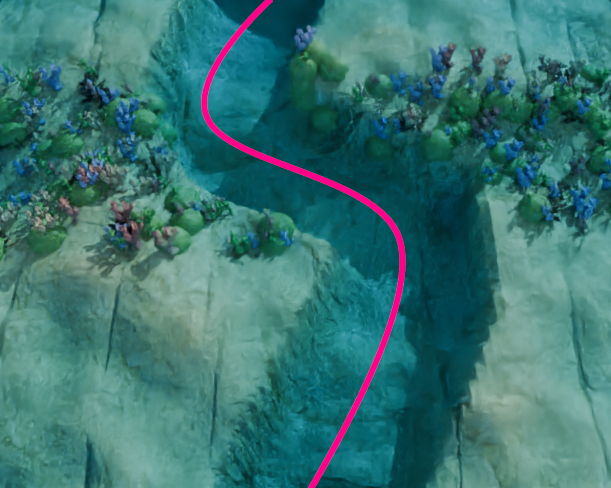
\includegraphics[width = 0.3 \linewidth]{Figures/Interactions/InteractionEdition1.png}
    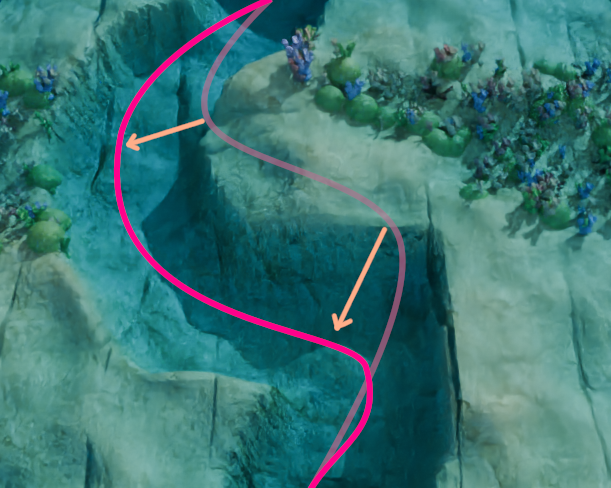
\includegraphics[width = 0.3 \linewidth]{Figures/Interactions/InteractionEdition2.png}
    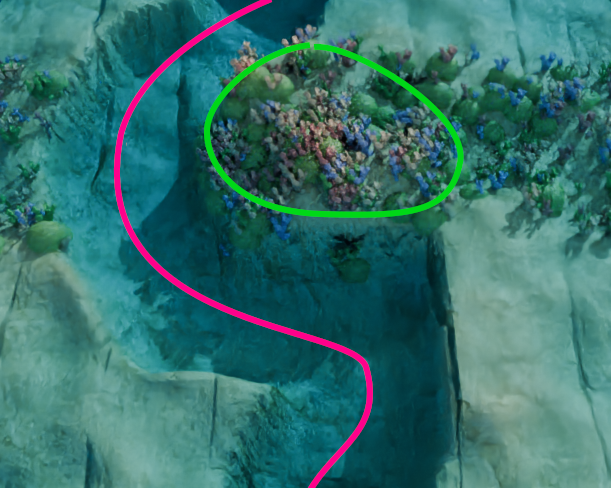
\includegraphics[width = 0.3 \linewidth]{Figures/Interactions/InteractionEdition3.png}
    \caption{Starting from a coral colony developed around a canyon (\textit{left}), the user edits the shape of the canyon, resulting in a different configuration of the scene, killing the corals that ends too deep in the water (\textit{center}) and the development and growth of new corals at the previous location of the canyon (\textit{right}). }
    \label{fig:semantic-representation_user-interaction}
\end{figure}

As long as a non-zero \gloss{FitnessFunc} is defined in the terrain, new \glosses{EnvObj} can be forced by the user at any point of the simulation. 

% \subsection{Guiding the simulation}
Control over the region of the terrain that should be updated can be given by adjusting all \glosses{FitnessFunc} through a scalar field $\influence: \R^2 \to \R $ such that the \gloss{FitnessFunc} $\fitnessFunc(\p)$ of any new \gloss{EnvObj} is evaluated as $\fitnessFunc^*(\p) = \influence{\p} \fitnessFunc(\p)$. This is especially useful in the planning of robotic simulations as we can first generate the overall shape of our terrain and secondly focus the generation process around the areas that may be visited by the robot, avoiding useless simulations and computer power. 
\cref{fig:semantic-representation_coral-colonization-scene} shows an example of colonization of the coral polyps that we limited manually into an annulus.
% \cref{fig:semantic-representation_focus-area-example} shows an example of colonization of the coral polyps that we limited manually.

% \begin{figure}
%     % \centering
%     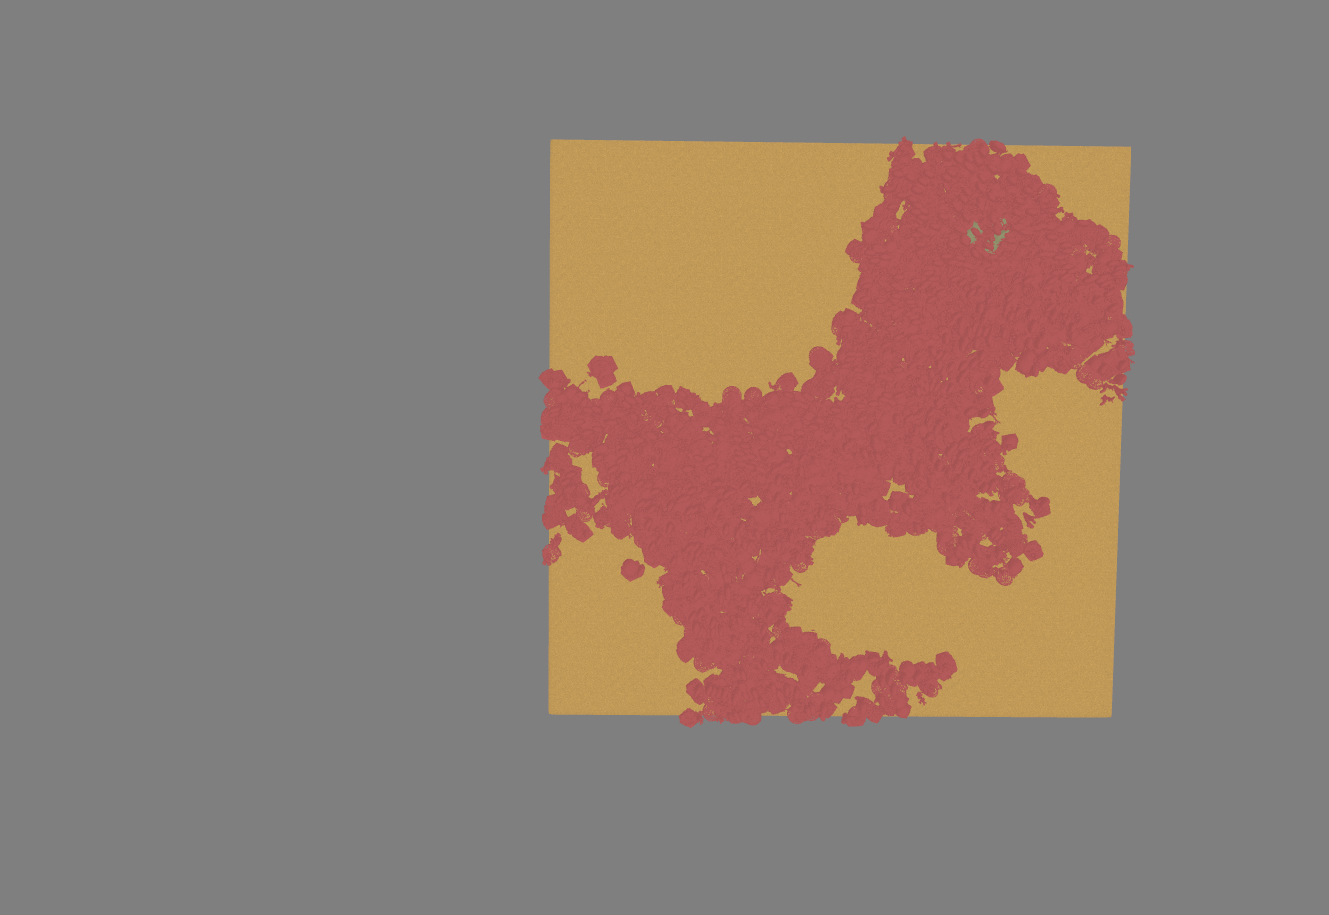
\includegraphics{Figures/UserControl/guidedGeneration1.png}
%     \caption{Controlling the generation area can produce a user-defined focused shape.}
%     \label{fig:semantic-representation_focus-area-example}
% \end{figure}

% - Changing the water currents

Our water current simulation is modeled as a simple vector field. As such, the user is able to interact with it at any moment of the simulation, allowing for the death of sensible \glosses{EnvObj} while it will guide the simulation into a new landscape. By modifying the water currents, the user also modifies the transport rate of \glosses{EnvMat} at this position. The modification of currents is given as a stroke, a parametric curve $\curve$ for which we evaluate $\Delta \Wuser(\p)$ just as for curved environment objects (\cref{sec:semantic-representation_water-currents}).

\subsection{Indirect interaction with \glosses{EnvObj}}
\label{sec:semantic-representation_events}
A configuration file can define in advance the different \glosses{GeoEvent} that should be triggered during the simulation. This can be useful to generate landscapes that are close to some existing locations. 
Multiple \glosses{GeoEvent} can be triggered either as sudden or continuous environmental changes. These changes play a huge role in the morphology of landscapes.
We define \glosses{GeoEvent} with a starting point and an ending point, such that at any time of the simulation we can compute the progress of the \gloss{GeoEvent} as $\tEvent \in [0, 1]$.

Water level changes are important \glosses{GeoEvent} that shape the underwater landscapes. As previously submerged \glosses{EnvObj} get elevated above water level, flora and fauna terrain features dry and die. Deprived from the living part of the features, everything is more affected by terrestrial erosion. By updating the value of the depth $\depth$ evaluated in the \glosses{FitnessFunc}, any \gloss{EnvObj} that is sensible to the depth will be impacted automatically, that may be causing death (\cref{fig:semantic-representation_water-event}). The modification of the water level is defined as 
\begin{align*}
    \depth(\p) = \depth_0(\p) + \sum_{e \in \events} \Delta \depth_e \tEvent
\end{align*}
with $\Delta \depth_e$ the amount of water rising or lowering during an \gloss{GeoEvent}. We assumed a linear evolution of the water level during an \gloss{GeoEvent}. This allows to evaluate the depth at any point in space and in time.

\begin{figure}
    % \centering
    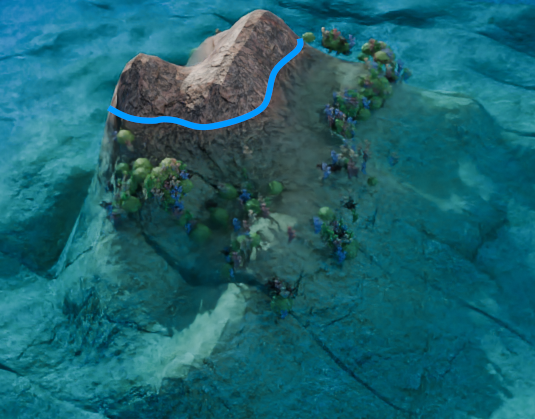
\includegraphics[width = 0.45 \linewidth]{Figures/Interactions/InteractionWater1.png}
    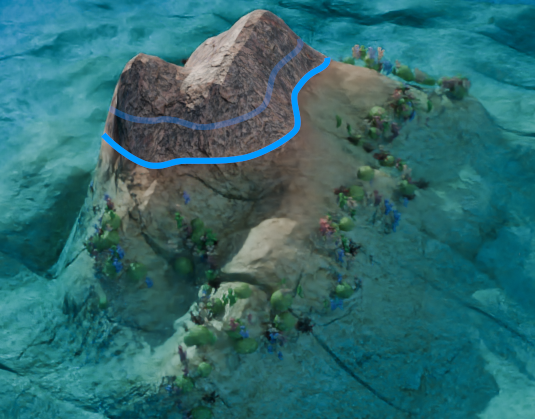
\includegraphics[width = 0.45 \linewidth]{Figures/Interactions/InteractionWater3.png}
    \caption{Lowering the water level by a few meters caused most of the coral objects to satisfy $\fitnessFunc \leq 0$, causing their death. Since the water level (blue) decrease slowly, new coral objects spawn progressively at a lower altitude.}
    \label{fig:semantic-representation_water-event}
\end{figure}

Subsidence and uplift are the main \glosses{GeoEvent} that create or destroy islands in the long term. These \glosses{GeoEvent} are simulated as a simple factor on the height field of the generated terrain (\cref{fig:semantic-representation_subsidence-event}). Subsidence is not always uniform in the terrain. As such, the user can provide a position $\q$ at which the subsidence is the strongest, the amount of subsidence applied $\Delta \height_e$ and a standard deviation $\std$ for which we can then compute at any point in space and time of the simulation the height of the terrain
\begin{align*}
    \height(\p) = \height_0(\p) \cdot \sum_{e \in \events}{G(\norm{\p - \q})} \Delta \height_e \tEvent 
\end{align*}
with $G(x)$ the Gaussian function
\begin{align*}
    G(x) = \exp \left(-\frac {x^{2}}{2 \std ^{2}}\right)
\end{align*}

\begin{figure}
    % \centering
    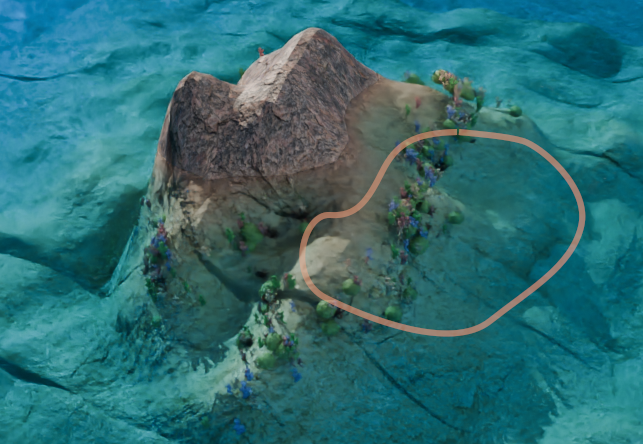
\includegraphics[width = 0.45 \linewidth]{Figures/Interactions/InteractionSubsidence1.png}
    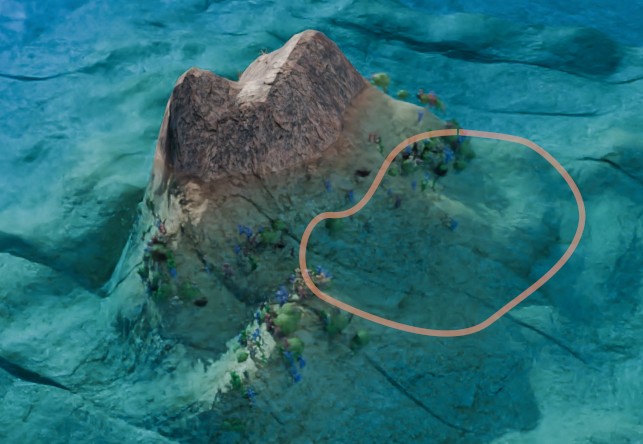
\includegraphics[width = 0.45 \linewidth]{Figures/Interactions/InteractionSubsidence2.png}
    \caption{Simulating subsidence on a part of the terrain (brown area) cause the depth value to change locally, resulting in the death of coral objects that find themselves too deep to survive. Here two subsidence \glosses{GeoEvent} are triggered in parallel. }
    \label{fig:semantic-representation_subsidence-event}
\end{figure}

Storms are factors of the geomorphology of coral reefs \cite{VilaConcejo2016, Oron2023} and coasts \cite{Dominguez2005, Cowart2010}. Due to the extreme wind and wave velocities coasts are highly eroded in a short time period and the more fragile corals near the water surface are broken, possibly causing breaches in the reefs and spreading polyps in the currents direction. While there are many factors at play to understand the apparition of storms and the hydrodynamics affecting it, we simplified the model of storms to the user as a single epicenter $\q$ with a wind velocity $\windVelocity$ and a standard deviation $\std$ representing the spread around the epicenter (\cref{fig:semantic-representation_storm-event}). The computation of water currents are then computed as 
\begin{align*}
    \Wuser(\p) = \Wuser^*(\p) + \sum_{e \in \events} {\windVelocity \frac{G(\norm{\p - \q}}{G(0)}}
\end{align*}
In this case, we did not include the linear factor $\tEvent$ as storms are usually conserving a constant force for the time of the few weeks or months of their occurrence. 

\begin{figure}
    % \centering
    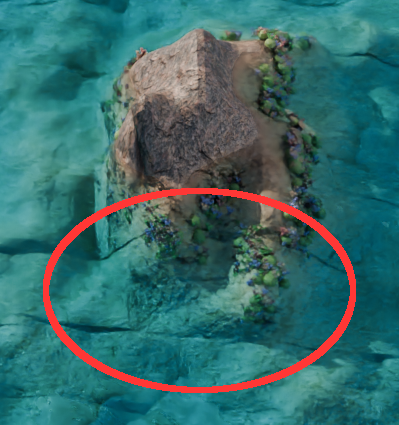
\includegraphics[width = 0.45 \linewidth]{Figures/Interactions/interactionStorm1.png}
    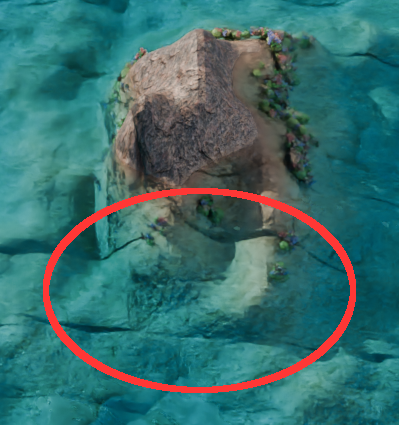
\includegraphics[width = 0.45 \linewidth]{Figures/Interactions/interactionStorm2.png}
    \caption{The result of a storm localized on one side of the island (red area) modifies the result of the evaluation of \glosses{EnvObj} around its epicenter for a short period of time. Most of the coral objects died from the \gloss{GeoEvent}, except few \glosses{EnvObj} less sensible to water currents strength. }
    \label{fig:semantic-representation_storm-event}
\end{figure}

% Just as for the rise and lowering of water level, the heat is modeled as a simple value of the environment. For shallow areas (<100m) we assume a linear relation between depth and temperature, and a constant value for the terrestrial environment. As such, we can model a heat wave by a change of the \glosses{EnvVal}. \Glosses{EnvObj} who are sensible to temperature may die instantly. The modification of the temperature is defined as 
% \begin{align*}
%     \temperature(\p) = T_0(\p) + \sum_{e \in \events} \Delta \temperature_e \tEvent + c \depth(\p)
% \end{align*}
with $\Delta \temperature_e$ the change of heat during an \gloss{GeoEvent}, $\temperature_0$ the temperature at the water surface, and $c$ a very small factor.

The framework can easily be extended as the \gloss{GeoEvent} system stays similar for all \glosses{GeoEvent}. Including higher level simulations in the \gloss{GeoEvent} system can be added, such as the simulation of tectonic activity, the use of fluid dynamics for tsunami \glosses{GeoEvent}, the integration of human activity, ...

\section{Results and discussion}
\label{sec:semantic-representation_results}
Our method provides a way to generate scenes at different scales. We demonstrate this capacity with the generation of a large scene of an island (\cref{fig:semantic-representation_teaser}) after what we focused the generation process in a canyon (\cref{fig:semantic-representation_canyon-scene}), then a small-scale visualization of coral colonies (\cref{fig:semantic-representation_coral-colonization-scene}).
In the examples, we rendered the \glosses{EnvObj} as a implicit tree or as individual meshes. The island, lagoons, reefs, canyons and sand ripples as implicit surfaces

% \subsection{Mid-scale}
% \label{sec:semantic-representation_mid-scale}
A canyon scene can be generated using our method. The water flow is affected by the curve of the canyon such that the currents are oriented in the direction of the curve's tangent.In this example, we force the position of arches to be inside the canyon. The arches deposits a material "rock deposit", which is the main element of the \gloss{FitnessFunc} of the Rock object. The "rock deposit" is slightly affected by water currents, but its mass make it highly affected by gravity. As such, rocks will spawn underneath arches. In reality, an arch is often created as part of a large coral boulder that sees the calcareous bottom part detached by the water currents, often resulting in an arch surrounded by big rocks and smaller rocks from the erosion of the first rocks.
As such, we define an \gloss{EnvObj} "Arch" with a \gloss{FitnessFunc} $\fitnessFunc_{arch}(\p) = 5 - d(canyon - \p) * \norm{\Water(\p)}$, an \gloss{EnvObj} "Rock" using $\fitnessFunc_{rock}(\p) = \material_{rock\_deposit}(\p)$ and Pebble using $\fitnessFunc_{pebble}(\p) = \material_{smaller\_rock\_deposit}(\p)$. Finally, sand ripples are simply described as curves appearing where there is a lot of sand available: $\fitnessFunc_{ripple}(\p) = \material_{sand}(\p)$.
Following these simple rules, \cref{fig:semantic-representation_canyon-scene} shows the emergence of details in the scene. 

% \subsection{Small-scale}
% \label{sec:semantic-representation_small-scale}
In this example we defined three different types of corals, coralA, coralB and coralC, to illustrate the possibility to model behaviours from the choice of \glosses{FitnessFunc}. Each of the coral types deposits a material "coral polyp" and "coral polyp A" ("coral polyp B" and "coral polyp C" respectively). By considering a \gloss{FitnessFunc} that minimize the ratio $\frac{\text{coral polyp}}{\text{coral polyp A}}$, we can see an emergent behavior of the three types of coral fighting for the space colonization.
\cref{fig:semantic-representation_coral-colonization-scene} shows the result of this simulation at three different interations. At the border between two colonies, none of the colonies make progression due to the amount of coral polyp specific from the other colony.

\begin{figure*}
    % \centering
    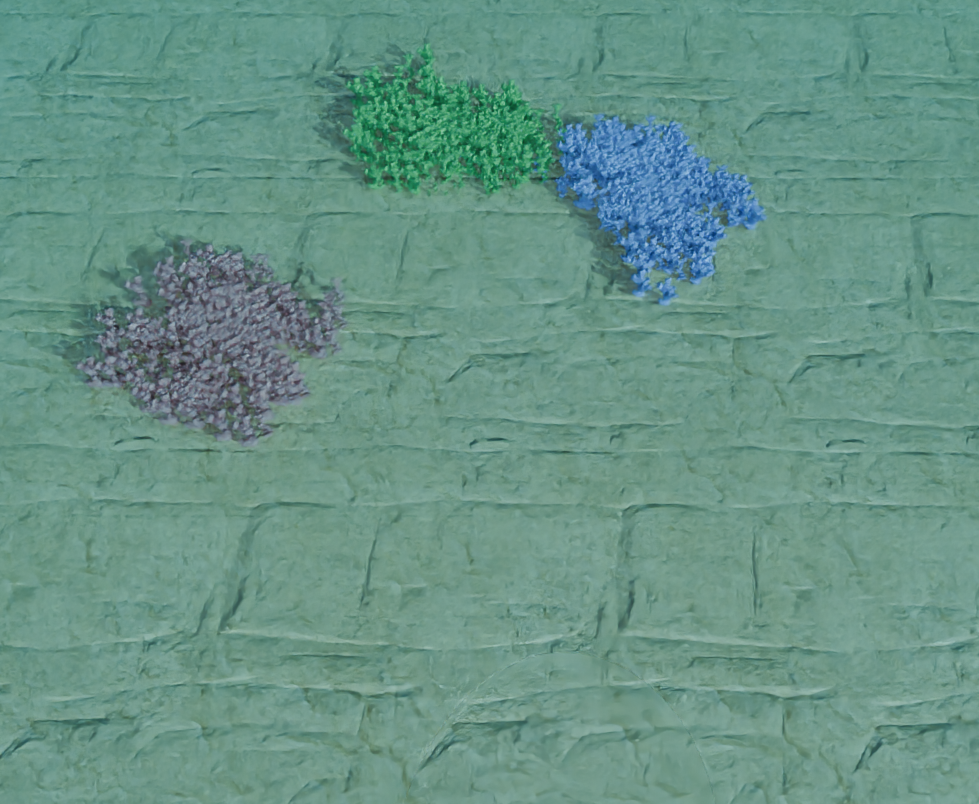
\includegraphics[width=0.24 \linewidth]{Figures/Colonization/col0.png}
    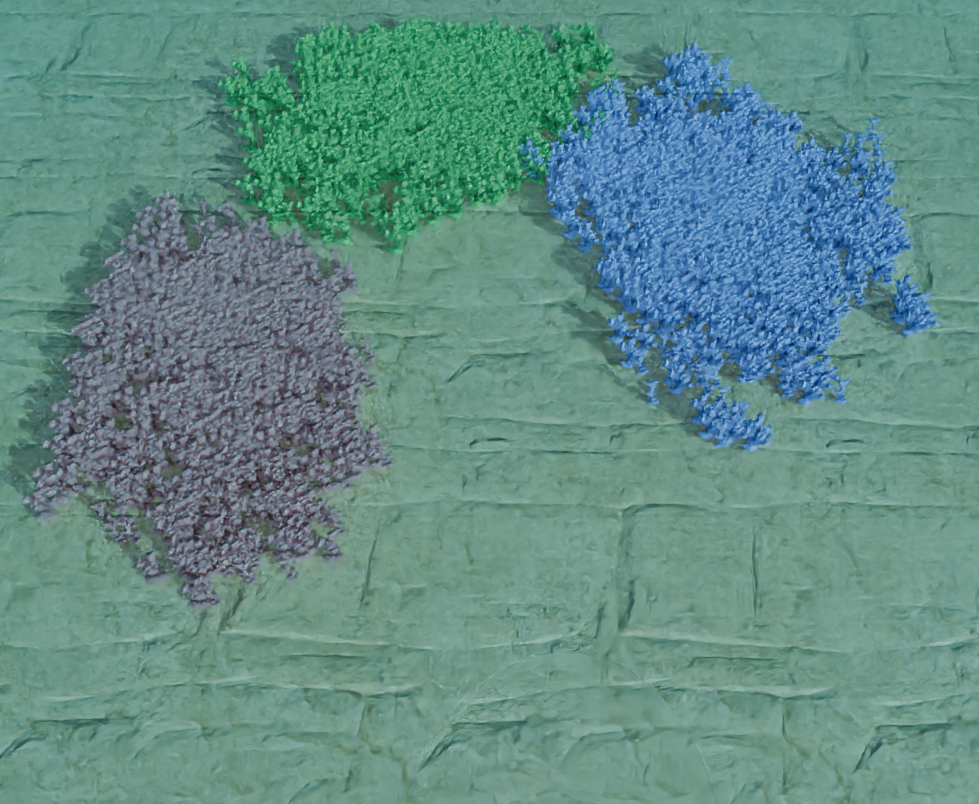
\includegraphics[width=0.24 \linewidth]{Figures/Colonization/col1.png}
    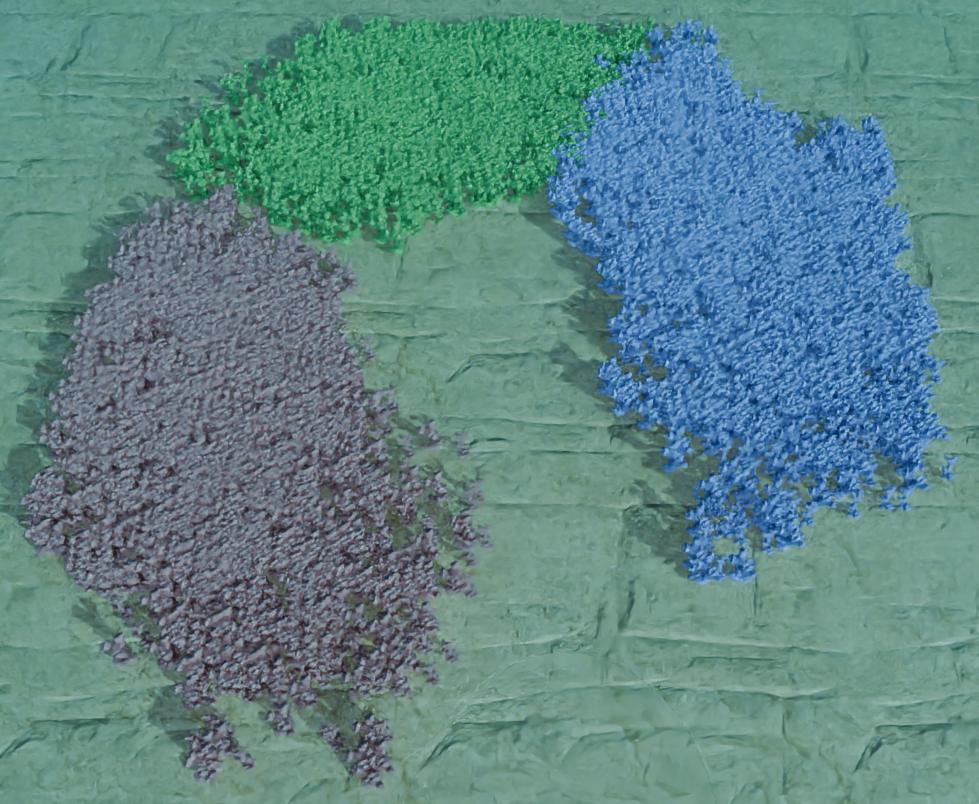
\includegraphics[width=0.24 \linewidth]{Figures/Colonization/col2.png}
    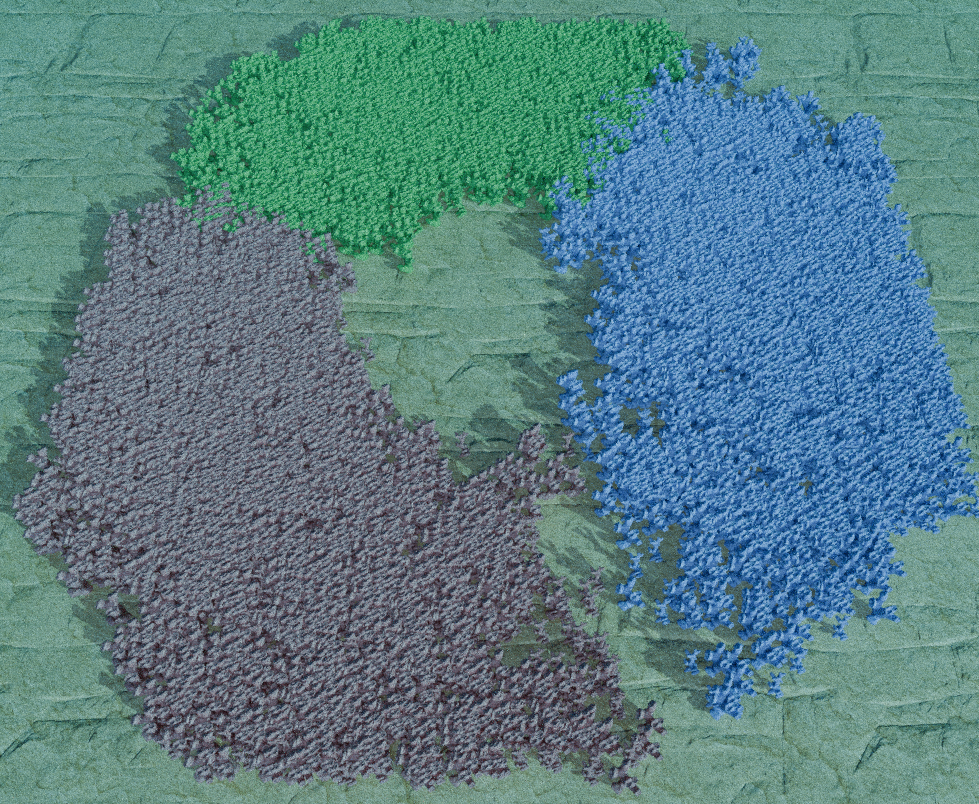
\includegraphics[width=0.24 \linewidth]{Figures/Colonization/col3.png}
    \caption{Three colonies of coral (red, blue, green) restricted to an annulus the middle section of the terrain fighting for the space.}
    \label{fig:semantic-representation_coral-colonization-scene}
\end{figure*}

\begin{figure*}
    % \centering
    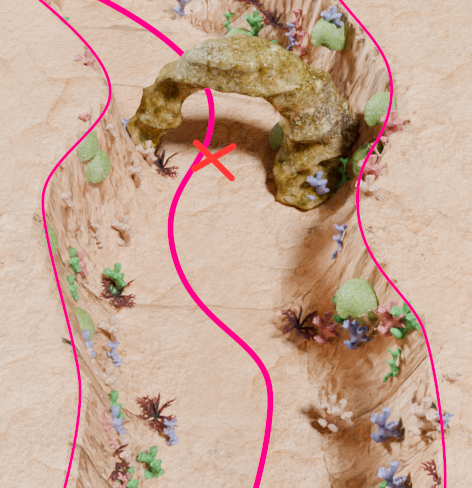
\includegraphics[width = 0.24 \linewidth]{Figures/Canyon/Canyon2.png}
    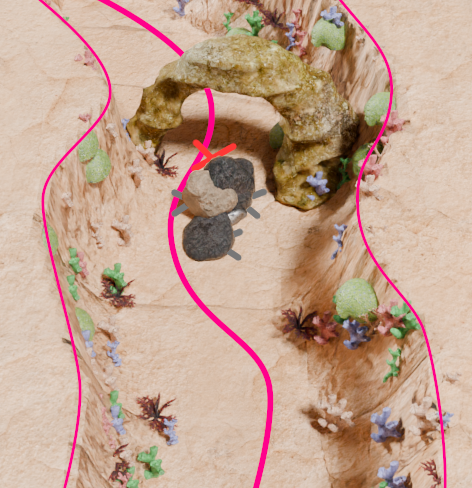
\includegraphics[width = 0.24 \linewidth]{Figures/Canyon/Canyon3.png}
    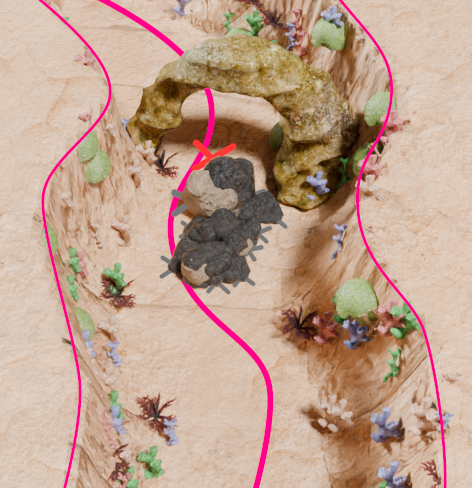
\includegraphics[width = 0.24 \linewidth]{Figures/Canyon/Canyon4.png}
    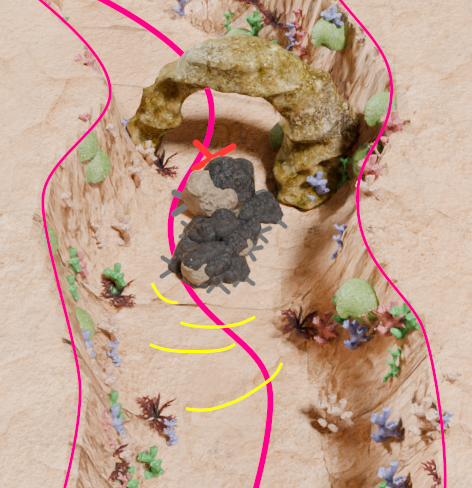
\includegraphics[width = 0.24 \linewidth]{Figures/Canyon/Canyon5.png}
    \caption{Evolution of a canyon scene at different iterations of the simulation. The apparition of an arch causes the spawning of rocks, pebbles, and finally some deposition of sand at the bottom of the canyon, spawning ripples. }
    \label{fig:semantic-representation_canyon-scene}
\end{figure*}


The proposed method aims to generate plausible landscapes using simplified versions of the evolution of an ecosystem and of the 3D representation. The biological realism of the result is highly correlated to the amount of simplification and assumptions, while the visual realism is completely dependent to the geometric functions used for the 3D modeling of the \glosses{EnvObj}. While proposing a flexible method that propose a generic approach for terrain generation, a close collaboration with fields experts and with graphists is needed to achieve optimal results.

Most simulation algorithm's quality depends on the size of the time step used, but with the introduction of a decay rate in the \glosses{EnvMat} properties, we limit the influence of time steps by considering that steady-state are reachable. The material deposition and absorption on punctual \glosses{EnvObj} can be seen as a Dirac function $\dirac$ centered at their position resulting in the advantage that material displacement function can use the definition of the diffusion equation instead of the advection-diffusion-reaction equation. This equation allowing us to evaluate the state of the material $\material$ without intermediate steps, but this is not applicable with curve- and region-based \glosses{EnvObj}. 

\section{Conclusion}
\label{sec:semantic-representation_conclusion}
We have proposed a method to generate terrains procedurally using sparse representations. This representation, the \glosses{EnvObj}, enables to introduce expert knowledge by the mean of the \glosses{FitnessFunc} that rule the \glosses{EnvObj} life cycle, but also to integrate the user in the loop during the generation process. We reduced the terrain resolution limitations by defining the environment objects as parametric features. Thanks to the sparse representation based on single points, curves and regions, we allow for direct manipulation of the \glosses{EnvObj} of the scene by the user which, thanks to the environment steady state consideration, also enables to include these interactions in the automatic simulation process.
Integrating environmental properties in the \gloss{FitnessFunc} of \glosses{EnvObj} allows the user to guide the generation through \glosses{GeoEvent}. Our method enables each \gloss{EnvObj} of the scene to influence the environment locally, reducing the need of computations while also retrieving \glosses{EnvVal} locally, which result in a parallelizable life-like simulation process. The genericity of the environment properties definitions should be sufficient for plausible generation of other landscape types as long as expert knowledge can be translated to \gloss{EnvObj}'s formalism.


We limited our work to the use of 2D scalar fields as they are more easily differentiable, interpretable and lighter than volumetric representations. However, future works include using 3D representations of the terrain and the environment to generate 3D terrains, including cavities, sub-terrestrial areas and the interior of coral structures. 
% The different possibilities to explore for this would be: the use of 3D particles to represent the state of the \glosses{EnvMat} in the environment, or voxel grids or flatten representation of the terrain's surface (but would not allow a different morphological shape than the height field...).

\begin{figure*}
    % \centering
    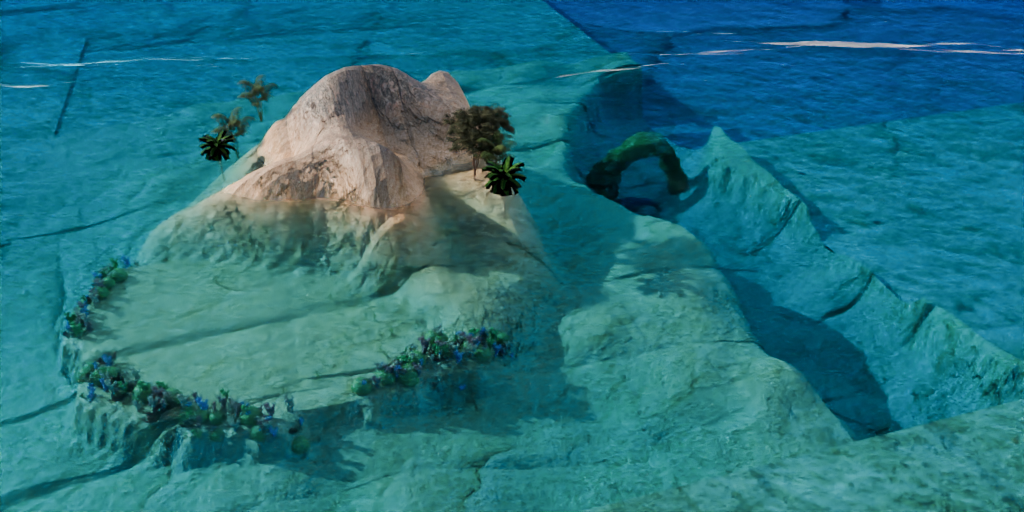
\includegraphics{Figures/CoralIsland/multiScene1 v2 final 1.png}
    \caption{A simple coral reef island is generated using an island, a lagoon, reefs coral polyps, beaches, trees and algae \glosses{EnvObj}. Trees appear on beaches and algae grow in the lagoon's sand. }
    \label{fig:semantic-representation_coral-island-scene}
\end{figure*}














% \section{Method}
% \label{sec:semantic-representation_method}
% The overall pipeline of the method is based on simple incremental generation like most rule-based systems. In this type of system, the final state is defined either by reaching equilibrium, or by verifying specific conditions, such as a maximum number of iterations. 
% We define our pipeline in three phases (\cref{fig:semantic-representation_pipeline}): the initialization phase that describe the generation and simulation rules, the iterative phase generating populating the terrain with our \glosses{EnvObj} and finally the output.


% \subsection{Pipeline overview}





















% \section{Expert knowledge integration}
% \label{sec:semantic-representation_biology}
%   The definition of the \glosses{FitnessFunc} of the \glosses{EnvObj} are inspired by the biological and geological factors that rule the evolution of underwater landscapes. The main factors are depth, light, water currents and biodiversity. External \glosses{GeoEvent} have direct and indirect repercussions on the biodiversity of underwater environments. Coral reef islands are complex bio systems in which fauna, flora and geology are mixed together. 

% \subsection{\Glosses{EnvObj} description}
% \label{sec:semantic-representation_represented-objects}
% We have represented with \glosses{EnvObj} some geologic features, animal features and flora features. The low island is most often raised in a circular shape as the process mainly appear around a hot spot under the ground. The evolution of an island into a coral reef island requires that the environmental conditions are sufficient for coral development: corals will grow slightly below the water surface as waves will break its growth and at a shallow depth (around 3m to 30m deep) in order for light to reach it. As coral grow and die, the skeleton is transformed into porous limestone, providing shelter to surrounding animals and reducing the impact of water erosion on the island. Corals drop polyps that are transported by the water flow and when they stick to a hard surface, as a rock or the reef itself, the coral may grow and colonize the area. As subsidence cause the island to lower, the living part of the coral reef keep growing toward light, which lead to a reef that is constantly close to the water level without reaching it due to wave erosion. The survival of reefs depends on the equilibrium between coral growth and and erosion. Eroded parts of the reef falling in the sheltered part of the reef accumulates, ending up by forming a lagoon. An island formed by a hot spot will inevitably subside in time, until it is completely flatten. As the coral reefs keep growing, only the lagoon remain, resulting in an atoll. \\
% In this work we we integrate the biological and geological knowledge in the \glosses{FitnessFunc} of the \glosses{EnvObj} we want to generate. We represent the islands as regions that can be appearing with a uniform distribution. From the formulation of the region description \eqref{eq:internal-energy-equation}, we mostly create circular islands. The coral features, \glosses{EnvObj} described as a single point, have a \gloss{FitnessFunc} that take into account the depth of the ground, the amount of sand, fresh water and polyps in their environment, as well as the strength of water currents. Each coral species have different living conditions, but we reduced our work to soft coral which are sensible to water strength and stony corals that are more resistant to erosion. Reefs are formed as coral's skeleton are transformed into calcareous stone, describing then as an \gloss{EnvObj} representing multiple others. 

% \subsection{Simplifications}
% \label{sec:semantic-representation_simplifications}
% The environmental factors simulated are greatly simplified as the real processes are in a very small time scale, that computer simulation are not able to simulate in interactive time. The use of \glosses{EnvObj} aim to represent a plausible results, while avoiding modeling the smaller scale \glosses{GeoEvent}. Examples of simplifications are the geometry and material of each \gloss{EnvObj}, which have an influence on the water currents through friction, the water currents represented as stationary flows, while the water flow dynamics are a complex system that may change completely at two different times of the day, the animal influence on the reefs that they transform by the ingestion and deposition of sediments, ...
